\chapter{Návrh a implementace algoritmu}
\label{ch:navrh}
V~této kapitole bude představen navržený způsob detekce příznaků onemocnění na sítnici lidského oka a jeho implementace. Protože sítnice obsahuje různé struktury (žlutá skvrna, slepá skvrna a cévy), které nepředstavují nálezy a mohly by nepříznivě ovlivnit výsledek, je potřeba je také detekovat a z~celého procesu detekce příznaků onemocnění je vynechat. Tímto způsobem se zvýší přesnost tohoto algoritmu. Pořadí jednotlivých podkapitol odpovídá postupu výpočtu algoritmu.

\section{Předzpracování}
Pokud se podaří úspěšně načíst konkrétní snímek, je před dalším zpracováním změněna jeho vzorkovací frekvence. Hlavním důvodem je urychlení výpočtu, kde pokud se sníží celkový počet pixelů, které se mají zpracovat, sníží se tím i množství výpočtů, které je potřeba vykonat. Další výhodou je nastavování parametrů pro jednotlivé výpočty. Pokud jsou všechny vstupní snímky převedeny do určitého intervalu rozlišení, není potřeba definovat tyto parametry pro příliš široké spektrum rozlišení. V~tomto případě byl zvolen interval šířky obrázků od 2500~pixelů do 900~pixelů. Pokud má nějaký vstupní snímek na šířku větší počet pixelů než 2500, je provedeno snížení jeho vzorkování. Pro vytvoření jednoho nového pixelu je zapotřebí čtyř pixelů původních. Tímto způsobem se rozlišení obrázku sníží na polovinu --- bude mít poloviční šířku i poloviční výšku. Naopak pokud je nějaký vstupní obrázek užší než 900~pixelů, je provedeno zvýšení jeho rozlišení na dvojnásobek. Pokud některý ze snímků spadá do tohoto intervalu, je ponechán beze změny.

Dalším krokem je určení výše zmíněných parametrů výpočtů. Patří mezi ně velikost matice pro filtrování při získávání masky pozadí (filtr 1) a velikost matice pro filtrování při dalším zpracování (filtr 2). Tyto parametry jsou určeny na základě tří kategorií, které jsou dány intervalem šířky vstupních snímků. Přehled těchto hodnot lze vidět v~tabulce \ref{tab:parameters}. Díky úpravě rozlišení vstupních obrázku by měly všechny spadat do jedné z~těchto kategorií.

\begin{table}[ht]
  \begin{center}	
    \begin{tabular}{|c|c|c|}
      \hline
      \makecell{\textbf{Šířka snímku}\\\textbf{(v pixelech)}} & \makecell{\textbf{Filtr 1}\\\textbf{(v pixelech)}} & \makecell{\textbf{Filtr 2}\\\textbf{(v pixelech)}} \\
      \hline
      2500--1951 & 9$\times$9 & 13$\times$13 \\
      \hline
      1950--1401 & 7$\times$7 & 11$\times$11 \\
      \hline
      1400--900  & 5$\times$5 &  9$\times$9  \\
      \hline
    \end{tabular}
  \caption{Přehled parametrů výpočtů algoritmu.}
  \label{tab:parameters}
  \end{center}
\end{table}

\section{Získání masky pozadí}
Hlavním důvodem proč je potřeba oddělit pozadí snímku od popředí je efektivita. Při vyloučení pozadí z~následujícího zpracování dojde k~urychlení celkového výpočtu. Dalším důvodem je nežádoucí šum, který se na pozadí může objevit a který by mohl nepříznivě ovlivnit detekci.

Pro automatické oddělení masky pozadí od oblasti sítnice je potřeba nejprve převést výchozí snímek do odstínů šedé, aplikovat na něj vyhlazování pomocí průměrování normalizovanou maskou o~velikosti dané filtrem 1 (viz tabulka \ref{tab:parameters}) a následně zvolit takovou hodnotu prahu, která toto oddělení umožní. U~některých obrázků však pozadí není čistě černé a při zvolené hodnotě prahu, která fungovala pro většinu obrázků, se nedařilo oddělit pozadí snímku od sítnice. Z~toho důvodu je tato hodnota vypočítána pro každý snímek zvlášť.

Nejprve se získají čtvercové oblasti z~každého rohu obrázku, kde délka strany každé oblasti je rovna velikosti jedné desetiny výšky snímku. Následně se vypočítá průměrná intenzita jednotlivých oblastí a poté se vypočítá průměr těchto čtyř intenzit. Nakonec se tento průměr zaokrouhlí a přičte se k~němu hodnota 5. Tímto se získá velikost prahu.

Následným prahováním dojde k~již správnému oddělení pozadí od popředí. Pokud se ale v~pozadí objevovaly určité objekty jako například označení snímku, je potřeba tyto nežádoucí prvky odstranit. To je provedeno pomocí vyhledání kontur v~získané masce, kde největší kontura patří sítnici. Ta se ponechá a ostatní kontury se vyřadí. Při porovnání obrázků \ref{pic:chap05_background_mask_default} a \ref{pic:chap05_background_mask} je na první pohled jasné, která část obrazu patří pozadí a která sítnici.

\begin{figure}[h]
  \begin{minipage}[c]{0.47\textwidth}
    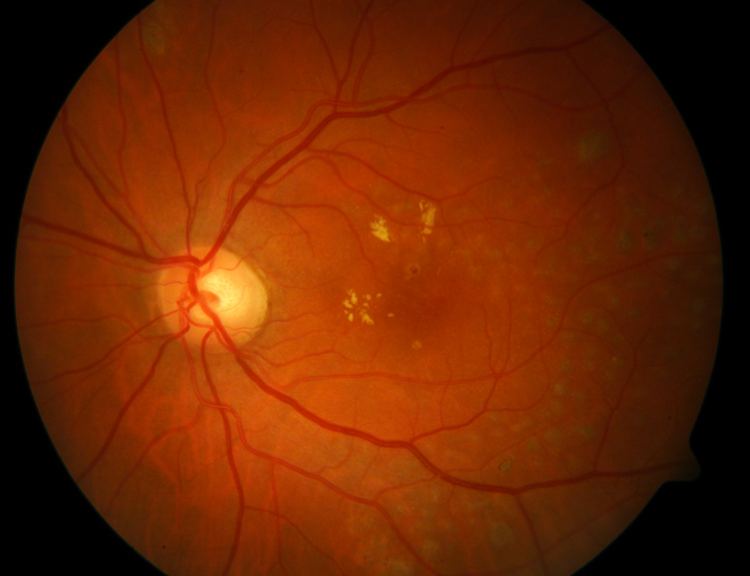
\includegraphics[width=\linewidth]{chap05_background_mask_default}
    \caption{Výchozí snímek.}
    \label{pic:chap05_background_mask_default}
  \end{minipage}
  \hfill
  \begin{minipage}[c]{0.47\textwidth}
    
\includegraphics[width=\linewidth]{chap05_background_mask}
    \caption{Maska pozadí.}
    \label{pic:chap05_background_mask}
  \end{minipage}
\end{figure}


\section{Získání vlastností oblasti sítnice}
Pro další výpočty u~algoritmů, které budou využity dále, je potřeba získat základní vlastnosti oblasti sítnice jako je střed a poloměr dané oblasti. K~jejich výpočtu je využita Houghova transformace pro hledání kružnic. Tento algoritmus pro extrakci vlastností je poměrně výpočetně náročný, ale vhodným nastavením mezních hodnot, kde se mají kružnice hledat, se celkový výpočet výrazně urychlí. Mezi tyto meze patří minimální vzdálenost mezi středy jednotlivých kružnic a dále minimální a maximální poloměr. Jako minimální vzdálenost mezi středy je zvolena větší hodnota z~počtu řádků a počtu sloupců snímku, kde se předpokládá, že požadovaná kružnice bude pouze jedna. Z~toho také vyplývá, že její průměr nemůže být větší než je počet těchto řádků nebo sloupců. Vydělením tohoto počtu dvěma získáme maximální poloměr. Minimální poloměr je vypočten ze vzorce pro obsah kružnice, kde je tento obsah dán velikostí oblasti sítnice. V~případě, že není dostupná maska pozadí a celý snímek je vyplněn sítnicí, pracuje se se středem snímku a jako poloměr je zvolena větší hodnota z~počtu řádků a počtu sloupců.


\section{Detekce optického disku}
Těžké exudáty vypadají podobně jako optický disk. Může se tedy stát, že při detekci dojde k~jejich záměně, a proto je potřeba ho detekovat a vyloučit z~dalšího zpracování. Optický disk je přibližně oválný útvar, který má na snímku sítnice často největší intenzitu. Díky této vlastnosti ho můžeme detekovat. Problém ale představují drúzy a exudáty, které mohou mít podobnou nebo dokonce větší intenzitu než optický disk. Z~tohoto důvodu se musí počítat i s~velikostí optického disku. Po experimentování nad databází snímků byl určen poloměr optického disku na hodnotu jedné sedminy poloměru oblasti sítnice. Hledá se tedy oblast s~určitou plochou nejjasnějších pixelů. 

Pro automatickou detekci optického disku je potřeba mít zpracovaný výchozí snímek. Z~něj se extrahuje zelený kanál, na kterém jde nejlépe vidět kontrast struktur na sítnici a jejího pozadí (viz obrázek \ref{pic:chap05_optic_disc_green_channel}). Z~něj se vypočítá oblast, ve které se bude hledat. Ta je tvořena pásem po celé šířce obrázku s~výškou odpovídající jedné pětině průměru oblasti sítnice. Tento pás lze vidět na obrázku \ref{pic:chap05_optic_disc_area}. Důvodem zmenšení oblasti, ve které se hledá optický disk, je eliminace nesprávných detekcí ve smímcích s~příliš velkým odleskem. Po získání této oblasti se provede vyhlazování pomocí průměrování normalizovaným filtrem 2 (viz tabulka \ref{tab:parameters}).

\begin{figure}[h]
  \begin{minipage}[c]{0.47\textwidth}
    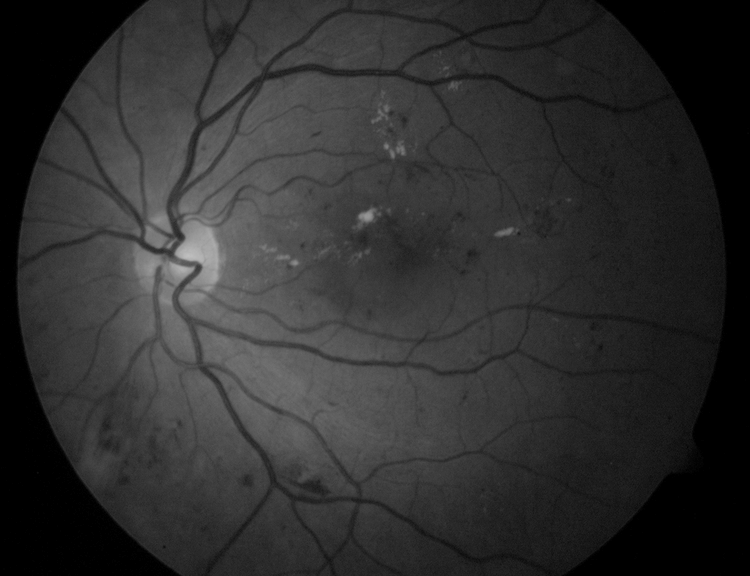
\includegraphics[width=\linewidth]{chap05_optic_disc_green_channel}
    \caption{Extrahovaný zelený kanál.}
    \label{pic:chap05_optic_disc_green_channel}
  \end{minipage}
  \hfill
  \begin{minipage}[c]{0.47\textwidth}
    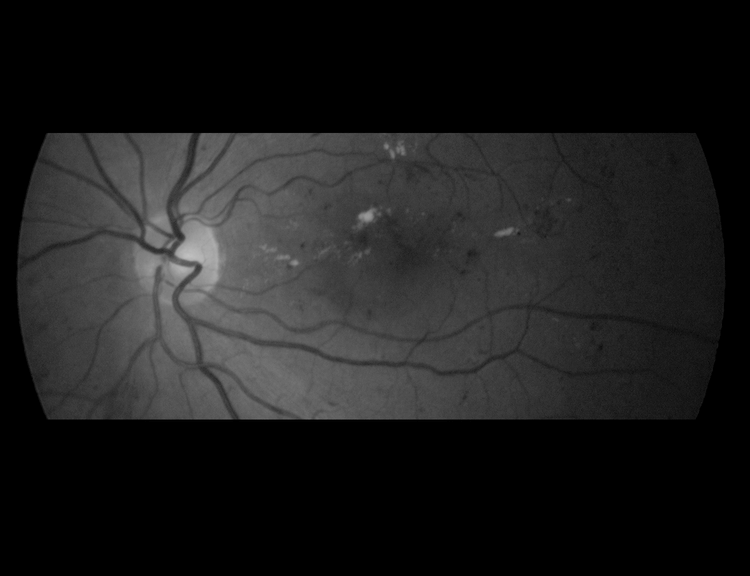
\includegraphics[width=\linewidth]{chap05_optic_disc_area}
    \caption{Zúžená oblast.}
    \label{pic:chap05_optic_disc_area}
  \end{minipage}
\end{figure}

Samotná detekce spočívá v~cyklickém binárním prahování, které začíná na maximální hodnotě 255 a postupně snižuje tento práh. Po každém prahování se ve snímku hledají kontury získaných oblastí, kterým se vypočítá jejich obsah. Kontuře, která obsahuje minimálně 11krát více pixelů než je poloměr oblasti sítnice, je vypočítána kružnice, která ji opisuje. Pokud je její poloměr menší nebo roven 1,2krát poloměru optického disku, pak mu tato oblast náleží. Těchto hodnot jsem dosáhl experimentováním nad databází snímků, kde vykazovaly největší úspěšnost. Výsledek posledního prahování je vidět na obrázku \ref{pic:chap05_optic_disc_thresh_area}.

Pomocí matematických momentů se vypočítá těžiště získané oblasti, které bude sloužit jako střed optického disku. Na základě umístění této oblasti se určí, zdali se jedná o~pravé či levé oko pacienta a podle toho se střed posune o~dvě pětiny svého poloměru daným směrem. Výsledek je na obrázku \ref{pic:chap05_optic_disc_result}.

\begin{figure}[h]
  \begin{minipage}[c]{0.47\textwidth}
    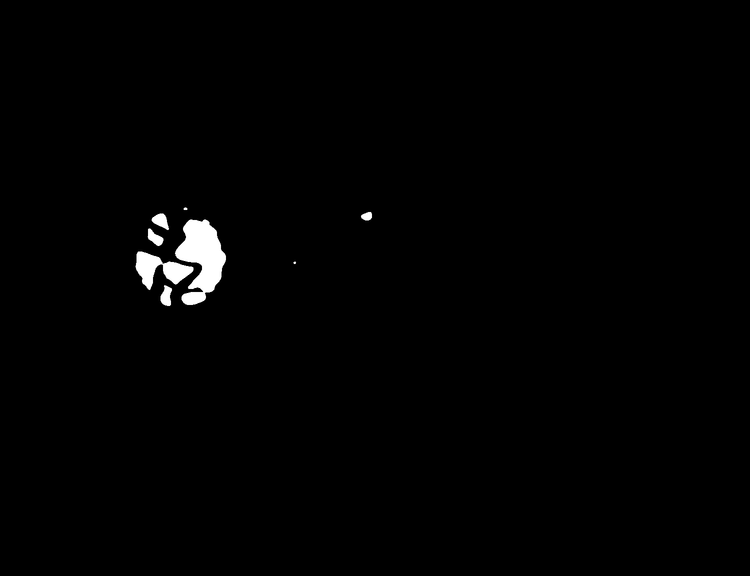
\includegraphics[width=\linewidth]{chap05_optic_disc_thresh_area}
    \caption{Konec binárního prahování.}
    \label{pic:chap05_optic_disc_thresh_area}
  \end{minipage}
    \hfill
  \begin{minipage}[c]{0.47\textwidth}
    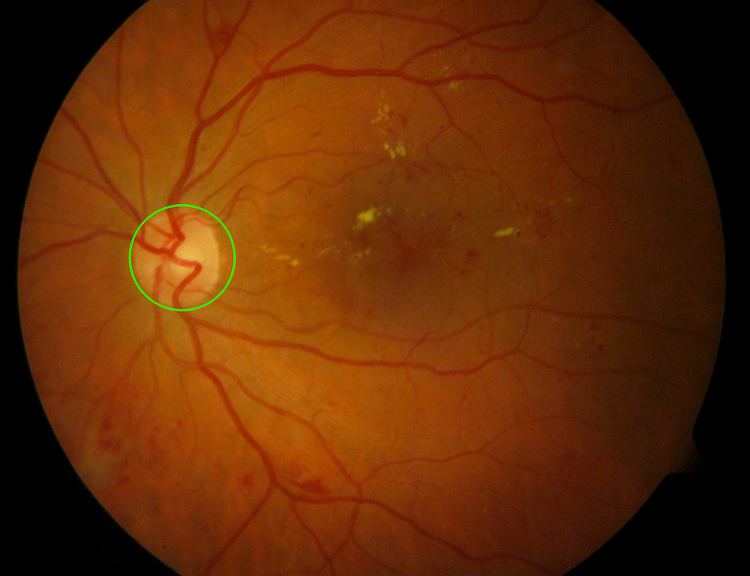
\includegraphics[width=\linewidth]{chap05_optic_disc_result}
    \caption{Detekovaný optický disk.}
    \label{pic:chap05_optic_disc_result}
  \end{minipage}
\end{figure}

Pro získání přesnější masky optického disku včetně menších oblastí, které mu náleží, se provádí dodatečné zpracování. Z~výchozího zeleného kanálu se extrahuje vypočítaná oblast optického disku (viz obrázek \ref{pic:chap05_optic_disc_mask_area}), která je průměrována normalizovanou maskou o~velikosti 5$\times$5~pixelů. Následně se provede jedno prahování s~hodnotou prahu o~2 nižší než je práh, při kterém došlo k~nalezení oblasti optického disku. Tímto způsobem se docílí daleko lepších výsledků. Rozdíl lze pozorovat na obrázcích \ref{pic:chap05_optic_disc_mask} a \ref{pic:chap05_optic_disc_mask_improved}.

\begin{figure}[h]
  \begin{minipage}[c]{0.315\textwidth}
    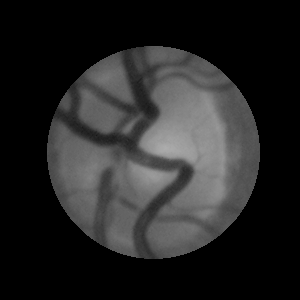
\includegraphics[width=\linewidth]{chap05_optic_disc_mask_area}
    \caption{Oblast optického disku.}
    \label{pic:chap05_optic_disc_mask_area}
  \end{minipage}
  \hfill
  \begin{minipage}[c]{0.315\textwidth}
    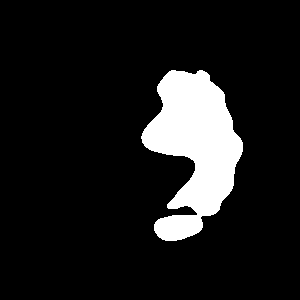
\includegraphics[width=\linewidth]{chap05_optic_disc_mask}
    \caption{Nalezená oblast.}
    \label{pic:chap05_optic_disc_mask}
  \end{minipage}
    \hfill
  \begin{minipage}[c]{0.315\textwidth}
    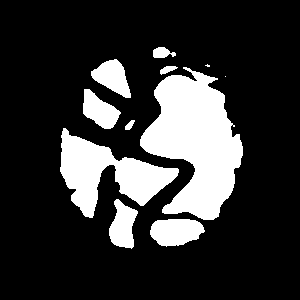
\includegraphics[width=\linewidth]{chap05_optic_disc_mask_improved}
    \caption{Výsledná maska.}
    \label{pic:chap05_optic_disc_mask_improved}
  \end{minipage}
\end{figure}


\section{Detekce fovey}
Abychom mohli správně klasifikovat příznaky VPMD, je potřeba detekovat foveu. Dalším důvodem, proč by se měla fovea detekovat, je možnost posouzení závažnosti onemocnění, neboť jak již bylo zmíněno dříve, fovea je struktura na sítnici představující místo nejostřejšího vidění. Díky tomu má největší vliv na kvalitu zraku a poškození právě této oblasti ji výrazně snižuje. Fovea je kruhovitá nebo oválná oblast, která je naopak oproti optickému disku jedním z~nejtmavších míst na sítnici. To v~některých případech může vést k~chybné detekci, kdy fovea splývá s~pozadím snímku nebo kdy je sítnice těžce poškozena. Na snímcích sítnice se fovea vždy vyskytuje relativně na stejném místě vzhledem k~optickému disku, a to přibližně ve dvou a půl násobku jeho šířky \cite{optic_disc}.

Při detekci fovey se opět pracuje se zeleným kanálem zdrojového snímku. Z~něho se vymezí zkoumaná oblast na základě posunutí středu optického disku pouze do vzdálenosti dvou a čtvrt násobku jeho průměru. Je to dáno tím, že poloměr optického disku je vypočítán tak, aby zahrnoval oblast o~něco větší, než je samotný disk. Poloměr zkoumané oblasti je pak 2krát větší než poloměr optického disku (viz obrázky \ref{pic:chap05_fovea_shift} a \ref{pic:chap05_fovea_area}). Zkoumaná oblast se následně vyhladí normalizovaným filtrem 2. Samotná detekce fovey je založená podobně jako u~detekce optického disku na cyklickém binárním prahování s~rozdílem, že hodnota prahu začíná na 0 a postupně se zvyšuje. Velikost hledané oblasti má i horní mez. Dolní mez je 6krát větší než poloměr oblasti sítnice a horní mez je 2,4krát větší než mez dolní. Tyto hodnoty byly získány také experimentováním nad databází snímků. První oblast, která spadá do těchto mezí, náleží fovey. Výsledek je zobrazen na obrázku \ref{pic:chap05_fovea_result}.

\begin{figure}[h]
  \begin{minipage}[c]{0.315\textwidth}
    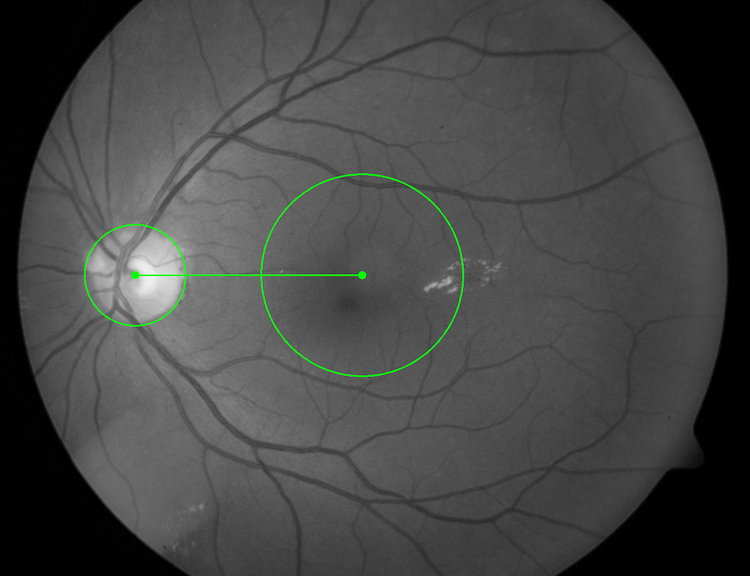
\includegraphics[width=\linewidth]{chap05_fovea_shift}
    \caption{Extrahovaný zelený kanál.}
    \label{pic:chap05_fovea_shift}
  \end{minipage}
  \hfill
  \begin{minipage}[c]{0.315\textwidth}
    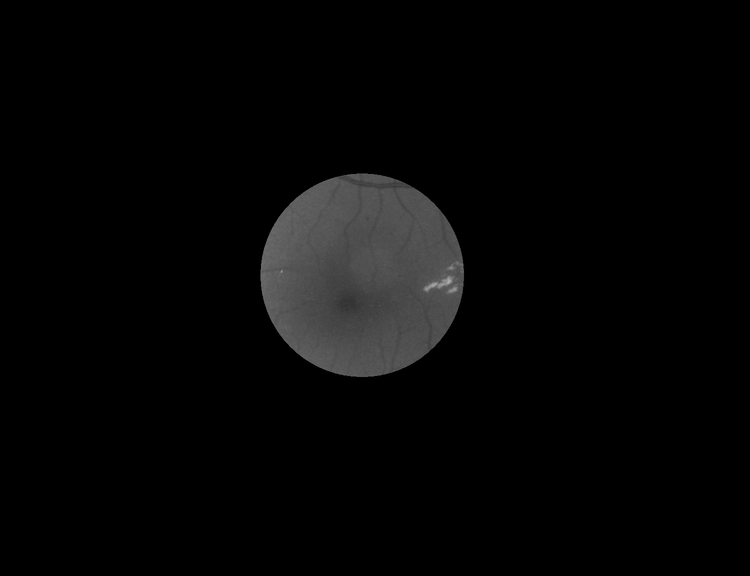
\includegraphics[width=\linewidth]{chap05_fovea_area}
    \caption{Vymezená oblast fovey.}
    \label{pic:chap05_fovea_area}
  \end{minipage}
    \hfill
  \begin{minipage}[c]{0.315\textwidth}
    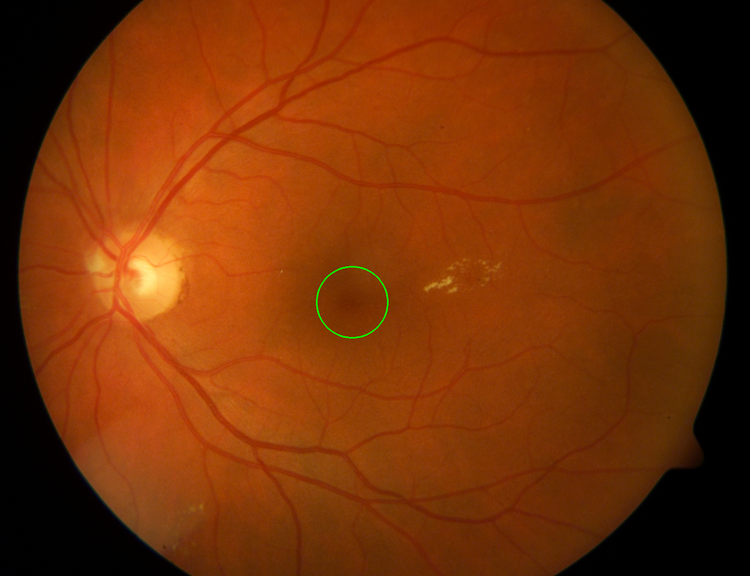
\includegraphics[width=\linewidth]{chap05_fovea_result}
    \caption{Výsledek detekce.}
    \label{pic:chap05_fovea_result}
  \end{minipage}
\end{figure}

\section{Detekce krevního řečiště}
Při detekci příznaků onemocnění na sítnici občas docházelo k~problému, kdy se některé části krevního řečiště jevily jako nález. Důvodem byla velikost dané cévy, její tvar, intenzita ve špatně osvětlených snímcích nebo při rozsáhlém poškození sítnice. Prvotním opatřením byla dodatečná kontrola, zdali se nejedná o~část krevního řečiště. Ta však nebyla příliš úspěšná, protože i přes to, že určitou část chybně detekovaných nálezů vyřadila, stále jich velké množství zůstalo. S~touto nízkou úspěšností bylo potřeba hledat řešení jinde. Velmi dobrých výsledků oproti předchozímu postupu bylo dosaženo při detekci krevního řečiště sítnice a jeho vyloučení ze získaných výsledků.

Jako první se na výchozí snímek (obrázek \ref{pic:chap05_blood_vessels_default}) aplikuje maska pozadí, která vyřadí oblast mimo našeho zájmu, a následně se extrahuje zelený kanál. Jak již bylo zmíněno, na zeleném kanále lze velmi dobře vidět kontrast pozadí sítnice a struktur nacházejících se na ní včetně krevního řečiště (viz obrázek \ref{pic:chap05_blood_vessels_green}). Na tento kanál se aplikuje Gaussovo adaptivní prahování, které transformuje obraz ve stupních šedi na binární obraz. Prahová hodnota se vypočítává jednotlivě pro každý pixel, kde se tento výpočet získá váženým součtem sousedních pixelů daného pixelu, od kterého se odečte určitá konstanta. Ta spolu s~velikostí okolí každého pixelu představuje parametry Gaussova adaptivního prahování. Čím je toto okolí menší, tím je tato metoda citlivější na drobné útvary a naopak čím je okolí větší, tím se tyto drobné útvary z~výsledku ztrácejí. Pokud je okolí pixelů příliš malé, do výsledků se začnou zahrnovat i oblasti, které nenáleží krevnímu řečišti a které mohou obsahovat i případné nálezy. Důležité tedy je zvolit velikost okolí tak, aby byl výsledek dostatečně podrobný a zároveň aby se nepřišlo o~příliš velké množství správných oblastí. Po experimentování s~různými snímky jsem tyto parametry zvolil 49 pro velikost okolí a 3 pro odečítanou konstantu. S~těmito hodnotami bylo dosaženo nejlepších výsledků (obrázek \ref{pic:chap05_blood_vessels_thresh}).

\begin{figure}[h]
  \begin{minipage}[c]{0.315\textwidth}
    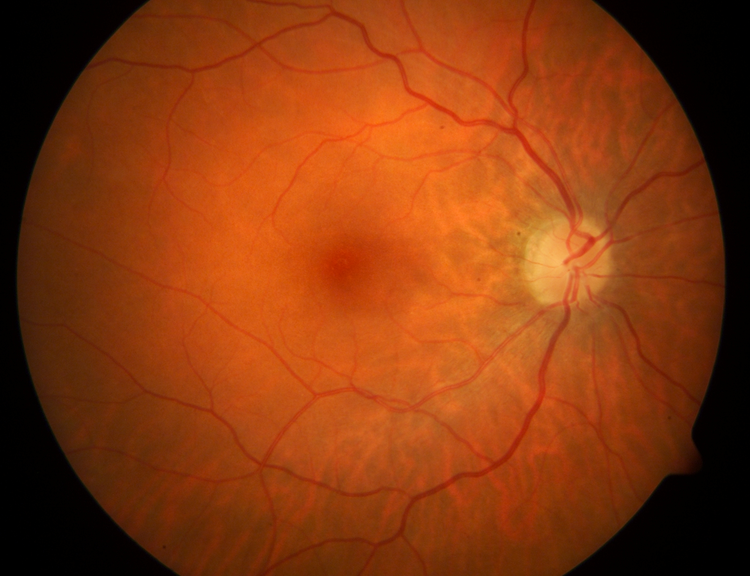
\includegraphics[width=\linewidth]{chap05_blood_vessels_default}
    \caption{Výchozí snímek sítnice.}
    \label{pic:chap05_blood_vessels_default}
  \end{minipage}
  \hfill
  \begin{minipage}[c]{0.315\textwidth}
    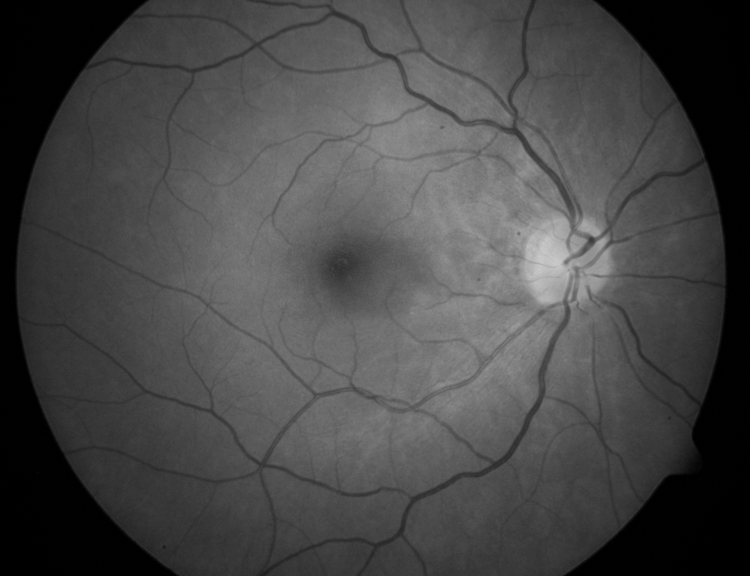
\includegraphics[width=\linewidth]{chap05_blood_vessels_green}
    \caption{Extrahovaný zelený kanál.}
    \label{pic:chap05_blood_vessels_green}
  \end{minipage}
  \hfill
  \begin{minipage}[c]{0.315\textwidth}
    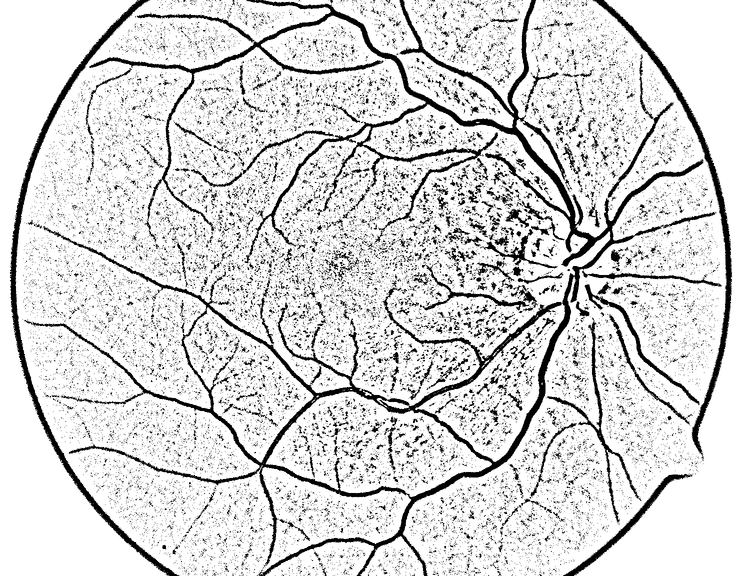
\includegraphics[width=\linewidth]{chap05_blood_vessels_thresh}
    \caption{Gaussovo adaptivní prahování.}
    \label{pic:chap05_blood_vessels_thresh}
  \end{minipage}
\end{figure}

Výstup prahování obsahuje i hraniční oblast mezi sítnicí a pozadím snímku, která byla nesprávně detekována. Této oblasti se zbavíme opětovným aplikováním masky pozadí. Nejprve se však snímek invertuje, protože to vyžaduje další zpracování, a pokud by se maska aplikovala jako první, došlo by i k~jejímu invertování a následně by se musela aplikovat znovu. Samotná maska se musí před jejím použitím upravit, protože hraniční oblast v~některých případech lehce zasahuje do oblasti sítnice. Aby se odstranila i tato přesahující část, provede se eroze sítnice v~masce. Výsledek tohoto zpracování lze vidět na obrázku \ref{pic:chap05_blood_vessels_inverted}.
Nyní následuje mediánové vyhlazování s~velikostí matice 5$\times$5, které redukuje šum typu sůl a pepř (viz sekce \ref{sec:smoothing}). Výsledný obraz ještě jednou podstoupí toto vyhlazování se stejnou maticí. To pomůže k~další redukci nežádoucích oblastí ze snímku (viz obrázek \ref{pic:chap05_blood_vessels_median}). 

\begin{figure}[h]
  \begin{minipage}[c]{0.47\textwidth}
    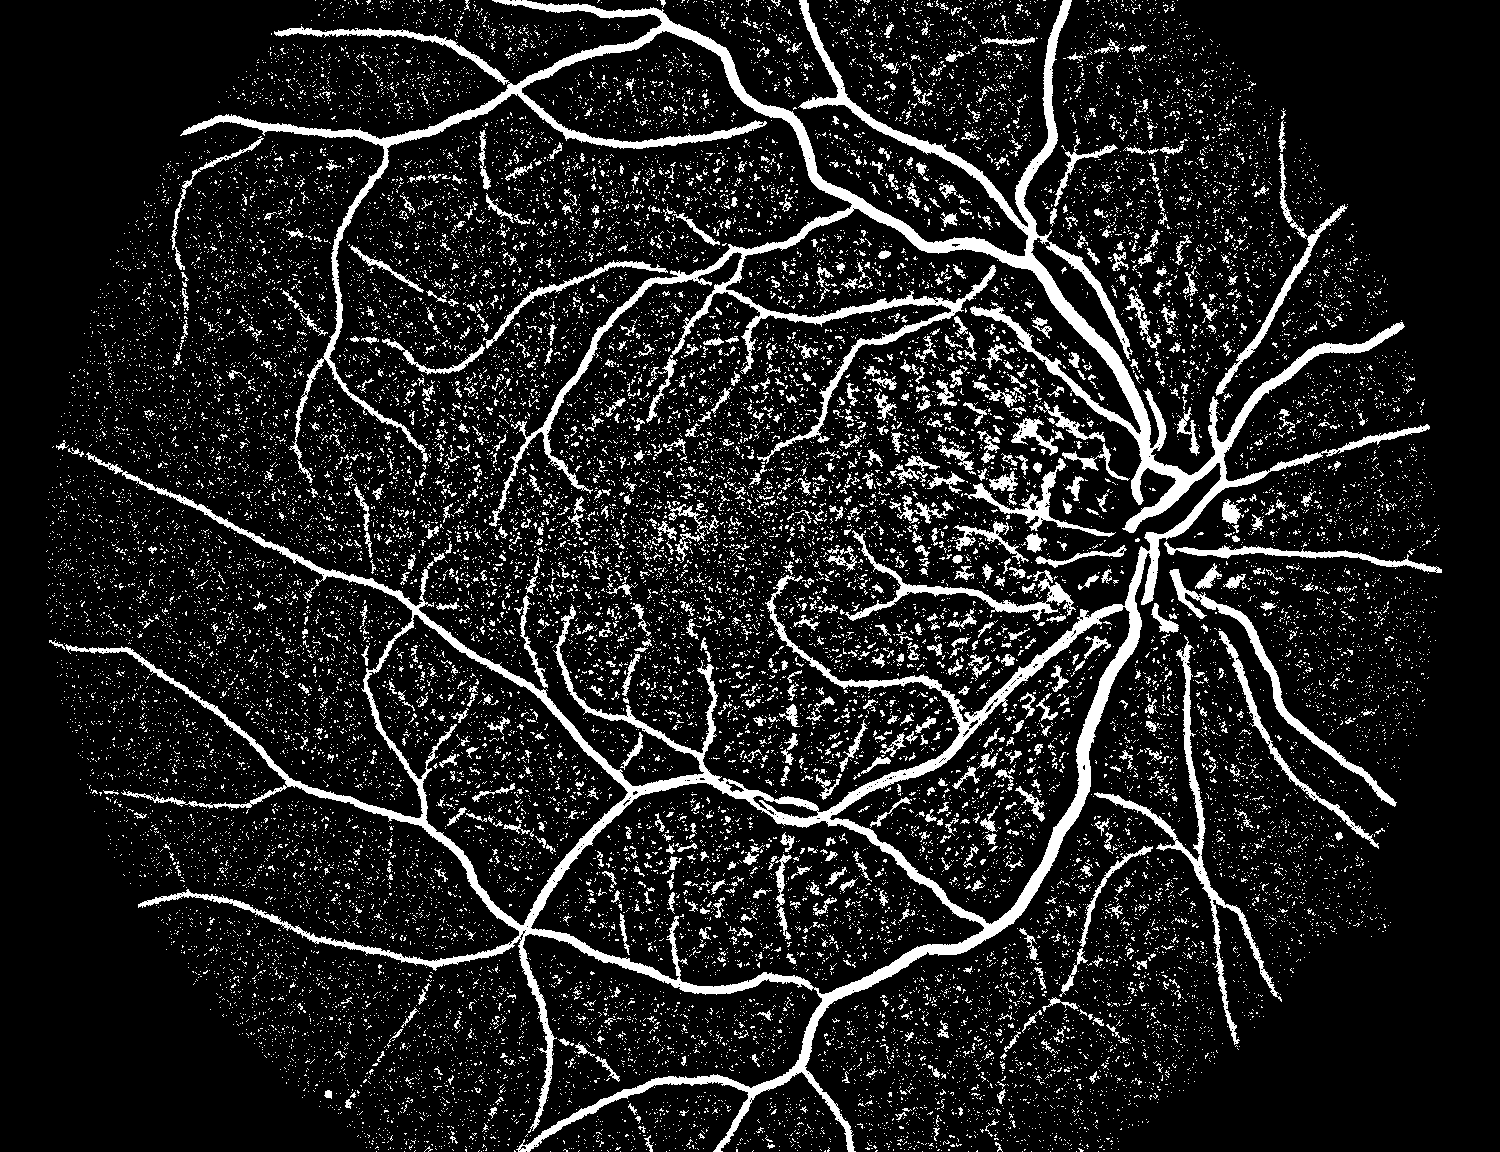
\includegraphics[width=\linewidth]{chap05_blood_vessels_inverted}
    \caption{Invertovaný výstup prahování.}
    \label{pic:chap05_blood_vessels_inverted}
  \end{minipage}
  \hfill
  \begin{minipage}[c]{0.47\textwidth}
    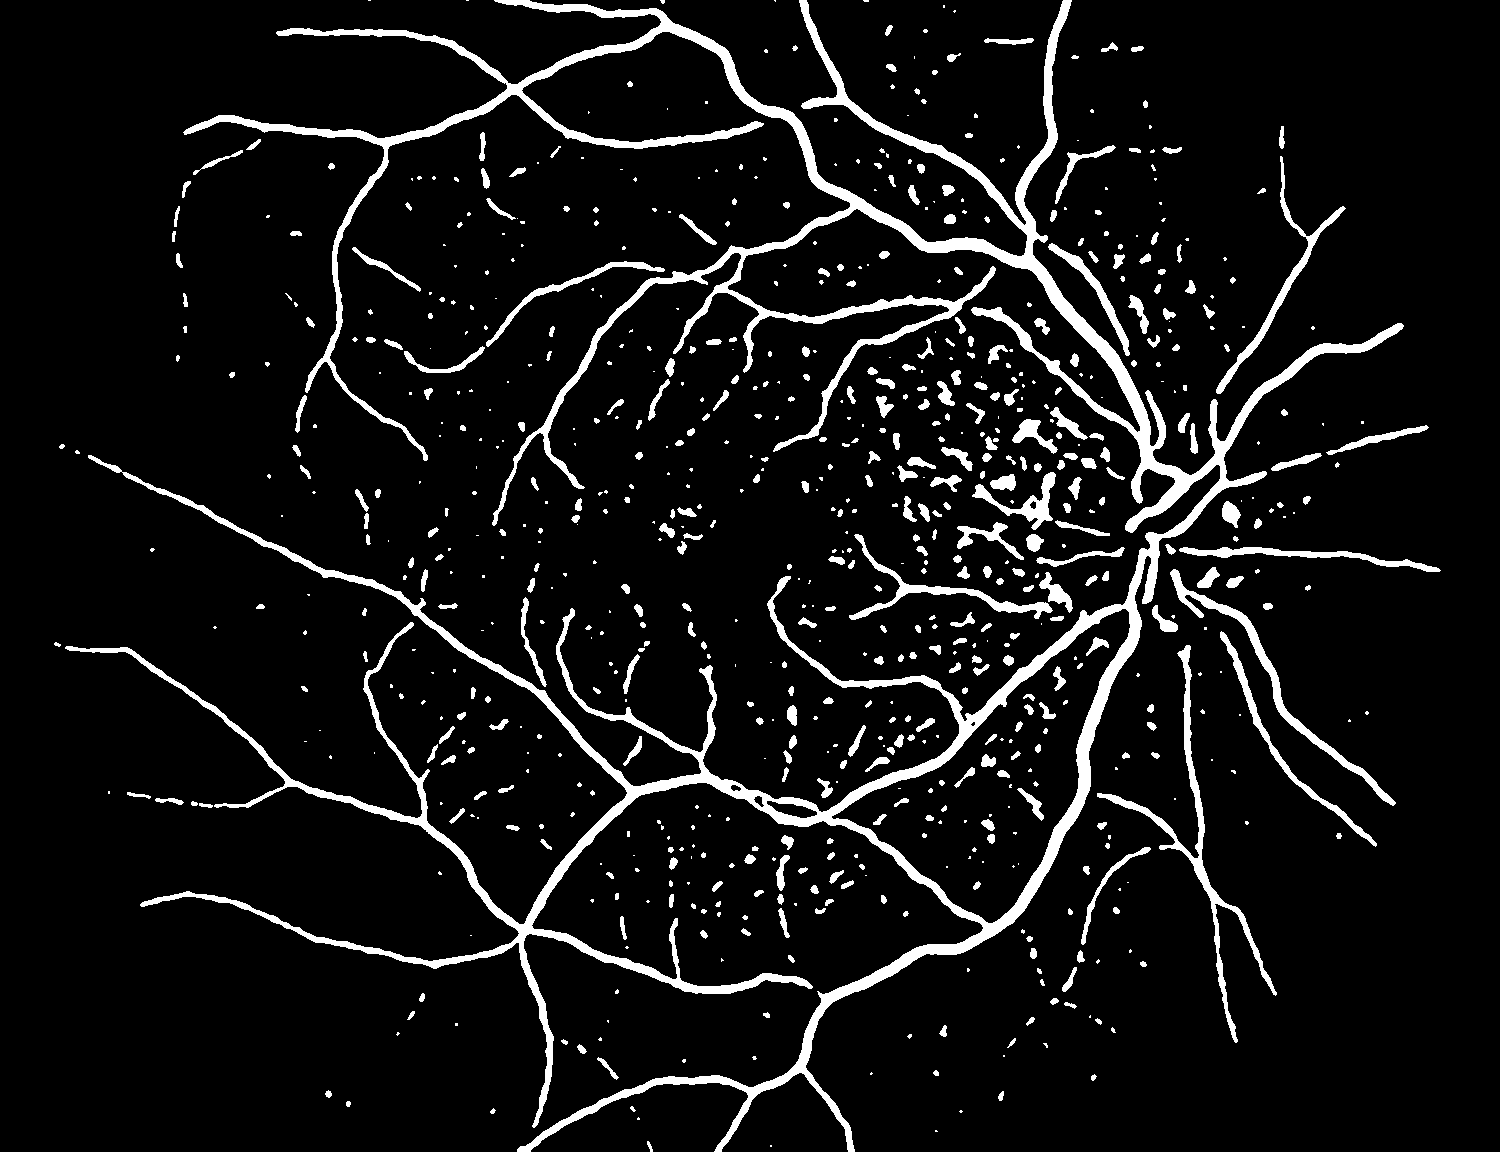
\includegraphics[width=\linewidth]{chap05_blood_vessels_median}
    \caption{Druhé mediánové vyhlazování.}
    \label{pic:chap05_blood_vessels_median}
  \end{minipage}
\end{figure}

Pro získání výsledné masky krevního řečiště se využívá semínkového vyplňování začínající na cévách v~optickém disku. Z~tohoto důvodu je potřeba vypočítat množinu počátečních bodů (semínek) a k~tomu jsou použity parametry optického disku, který byl již detekován. Nejprve se vytvoří nová maska obsahující kružnici kolem optického disku, která se následně bitově vynásobí výstupem z~Gaussova adaptivního prahování. Na nově získané masce se nyní pomocí Houghovy transformace detekují přímky. V~oblasti optického disku mají cévy největší průměr, proto se této vlastnosti využije při hledání těchto přímek specifikováním jejich minimální délky. Nyní už je na řadě semínkové vyplňování, u~kterého se jako počáteční body využijí středy detekovaných přímek. Výsledek po této operaci je viditelný na obrázku \ref{pic:chap05_blood_vessels_flood_fill}.

Při adaptivním prahování a vyhlazování původního snímku v~procesu detekce krevního řečiště může dojít k~porušení spojitosti cév a tím pádem nejsou některé části krevního řečiště zahrnuty ve výsledné masce. Abychom zamezili ztrátám těchto cév, maska (viz obrázek \ref{pic:chap05_blood_vessels_missed}), ze které bylo semínkovým vyplňováním extrahováno krevní řečiště, podstoupí dalšímu zpracování. To zahrnuje nalezení zbylých oblastí a jejich klasifikace, na jejímž základě se rozhodne, zdali se jedná o~část krevního řečiště nebo jiného objektu. První zkoumané kritérium je obsah dané oblasti. Pokud je obsah větší než 4500, vypočítá se poměr stran nejmenšího obdélníku ohraničujícího danou oblast, a pokud je tento poměr větší nebo roven 8, jedná se o~část cévy, jinak se zahazuje. Pokud je obsah větší než 1600, ponechávají se oblasti s~poměrem stran větším než 10, jinak se vypočítá průměrná šířka této oblasti, a pokud je menší než 6,8 (což by zhruba odpovídalo šířce cévy), oblast zůstává, jinak se zahazuje. Pokud je obsah větší než 300, opět se vypočítá poměr stran pro danou oblast, a pokud je větší nebo roven 5, jedná se o~součást cévy, jinak se zahazuje. Ostatní oblasti s~obsahem menším než 300 se zahazují. Celkový výsledek detekce krevního řečiště je zobrazen na obrázku \ref{pic:chap05_blood_vessels_result}.

\begin{figure}[h]
  \begin{minipage}[c]{0.315\textwidth}
    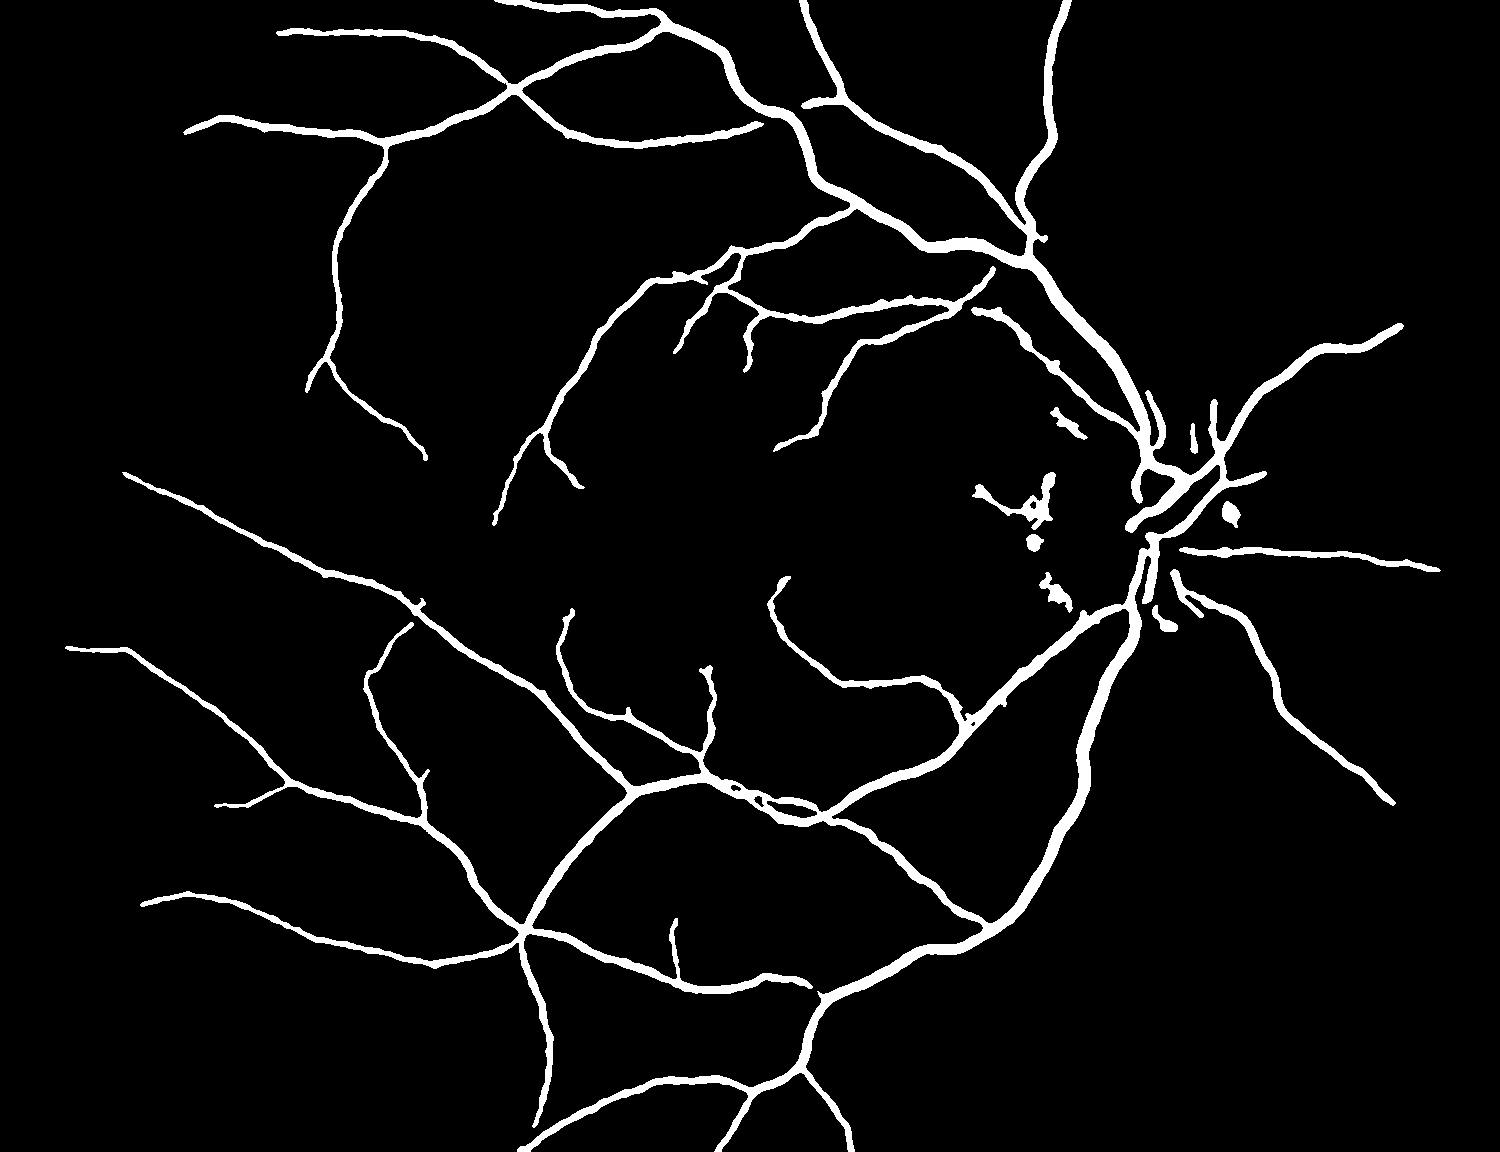
\includegraphics[width=\linewidth]{chap05_blood_vessels_flood_fill}
    \caption{Výsledek semínkového vyplňování.}
    \label{pic:chap05_blood_vessels_flood_fill}
  \end{minipage}
  \hfill
    \begin{minipage}[c]{0.315\textwidth}
    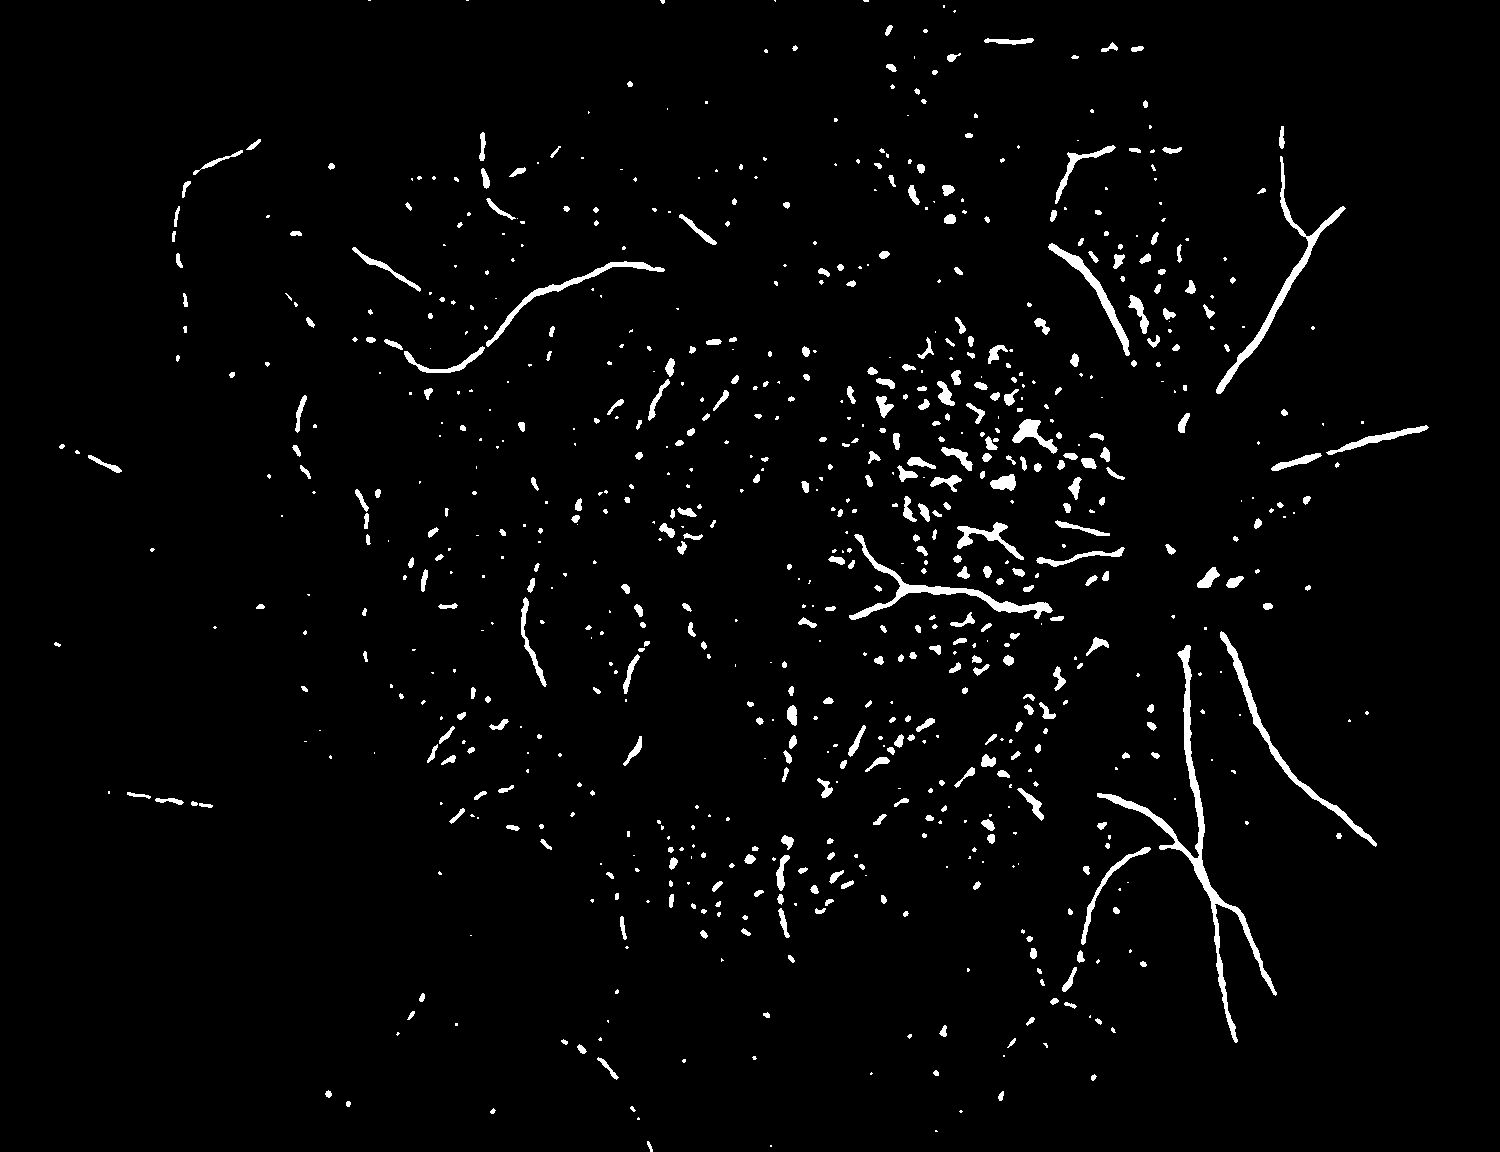
\includegraphics[width=\linewidth]{chap05_blood_vessels_missed}
    \caption{Maska s~vynechanými cévami.}
    \label{pic:chap05_blood_vessels_missed}
  \end{minipage}
  \hfill
  \begin{minipage}[c]{0.315\textwidth}
    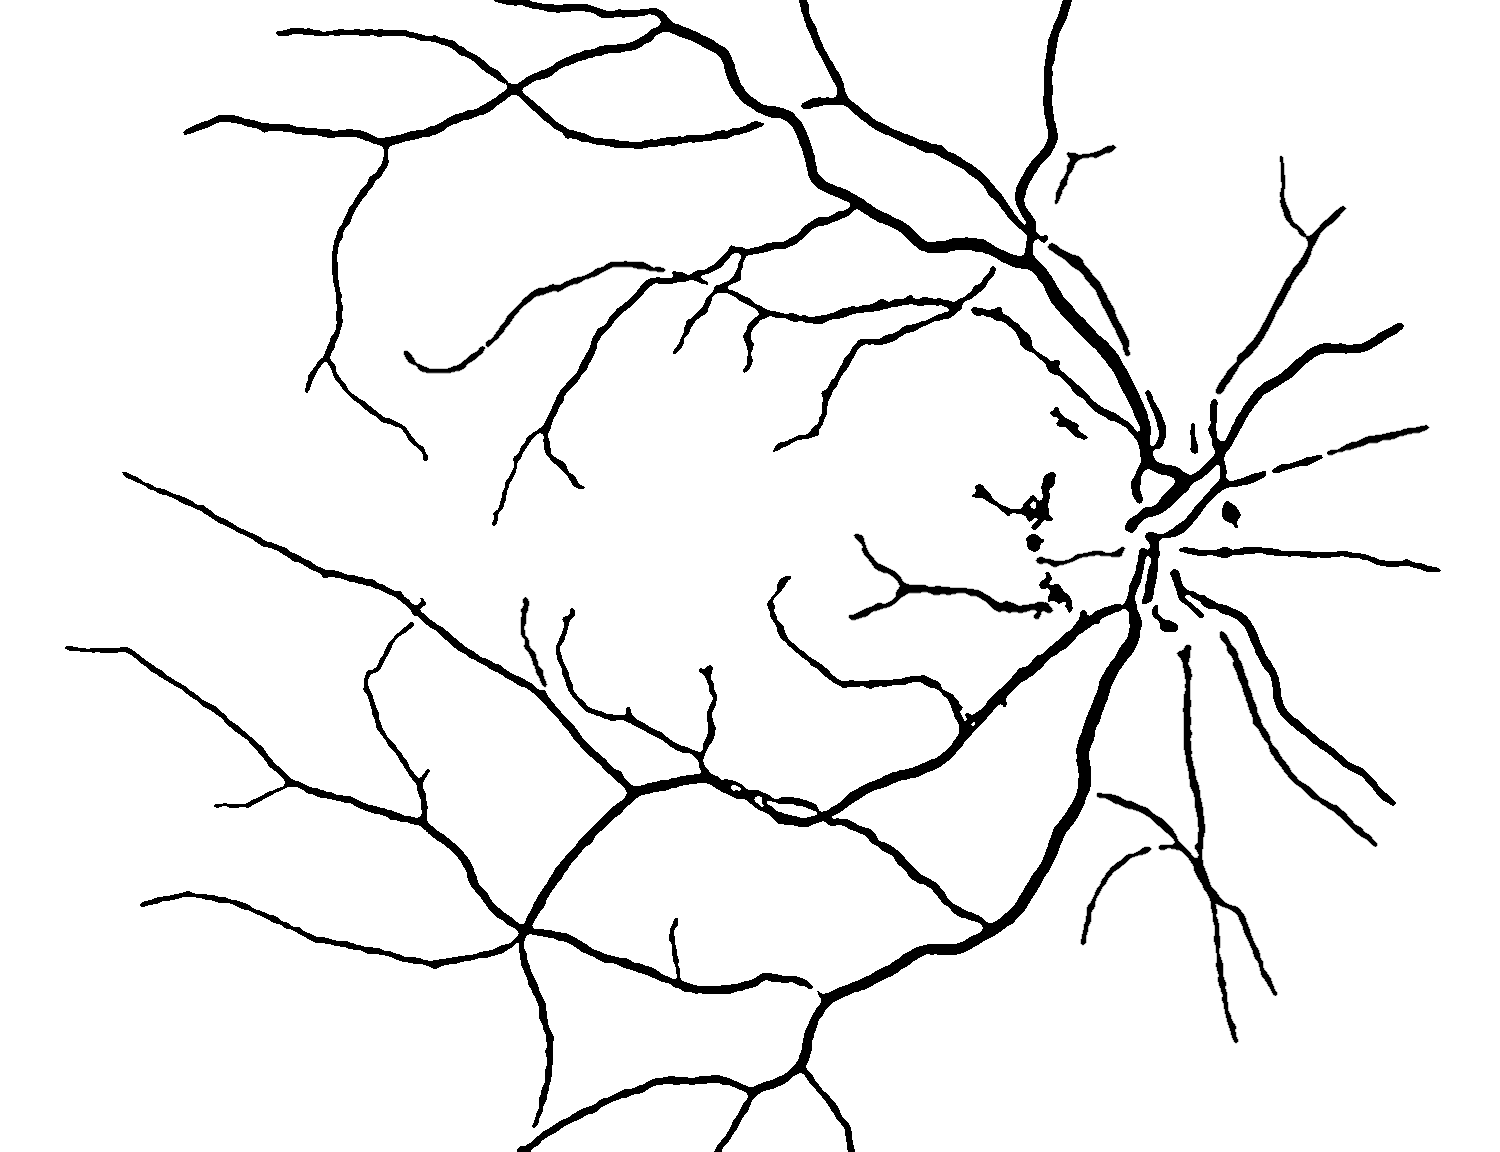
\includegraphics[width=\linewidth]{chap05_blood_vessels_result}
    \caption{Výsledek detekce krevního řečiště.}
    \label{pic:chap05_blood_vessels_result}
  \end{minipage}
\end{figure}


\section{Detekce drúz a exudátů}
Vzhledem k~nedostatku snímků s~VPMD při vytváření této práce se využijí i snímky s~exudáty. Drúzy vznikající při VPMD jsou velmi podobné těmto exudátům, které vznikají při diabetické retinopatii. Z~tohoto důvodu je možné detekovat tyto nálezy stejným algoritmem. V~obou případech se jedná o~tukové látky usazující se na sítnici, které mají žlutou barvu s~vysokou intenzitou. Jejich počet, tvar, velikost a umístění na sítnici se liší u~každého pacienta (viz kapitola \ref{ch:nemoci}).

\subsection*{Vymezení podezřelých oblastí}
Při detekci drúz a exudátů se opět pracuje se zeleným kanálem (obrázek \ref{pic:chap05_disease_green}) výchozího snímku (obrázek \ref{pic:chap05_disease_default}). Na něj je použito normalizované rozmazání s~maskou o~velikosti 7$\times$7~pixelů. Je to z~důvodu, aby se vyloučili drobné nevýrazné oblasti, které jsou někdy obtížné klasifikovat i zkušeným oftalmologem. Nad tímto rozmazaným snímkem se následně provede Gaussovo adaptivní prahování, které je velmi účinné pro vymezení podezřelých oblastí. Jak již bylo zmíněno výše, prahová hodnota u~Gaussova adaptivního prahování se vypočítává jednotlivě pro každý pixel, kde se tento výpočet získá váženým součtem sousedních pixelů daného pixelu, od kterého se odečte určitá konstanta. V~tomto případě je velikost okolí 5~pixelů a odečítaná konstanta je 0, tedy se nic neodečítá. Výsledek tohoto prahování lze vidět na obrázku \ref{pic:chap05_disease_threshold}. Teprve nyní se může aplikovat maska obsahující oblasti krevního řečiště a optického disku, které již byly detekovány dříve. Pokud by tato maska byla použita hned na začátku, nepříznivě by ovlivnila toto prahování, protože by v~obraze vznikl příliš velký kontrast mezi vyloučenými oblastmi a zbylou částí sítnice. To by způsobilo zahrnutí obrysů cév a optického disku do podezřelých oblastí, což je nežádoucí. Po aplikaci masky obraz následně podstoupí mediánovému vyhlazení s~velikostí matice 5$\times$5, aby se z~něj odstranil šum. Výsledné podezřelé oblasti jsou zachyceny na obrázku \ref{pic:chap05_disease_suspect}.

\begin{figure}[h]
  \begin{minipage}[c]{0.47\textwidth}
    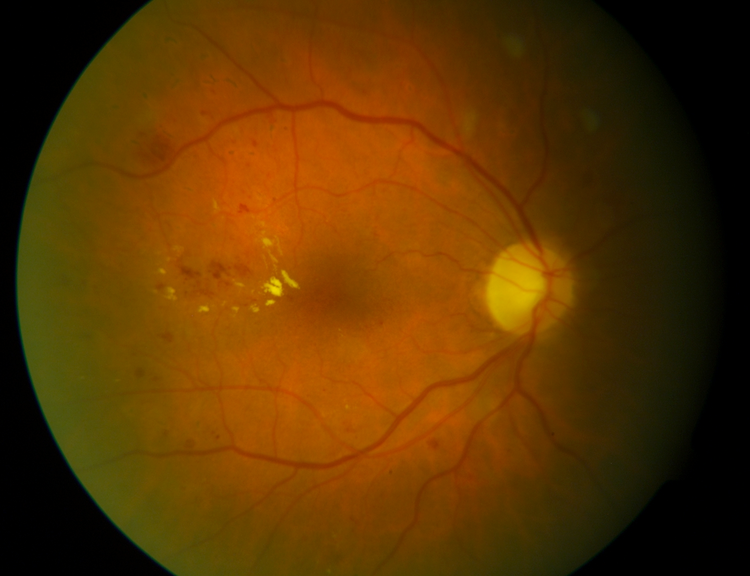
\includegraphics[width=\linewidth]{chap05_disease_default}
    \caption{Výchozí snímek.}
    \label{pic:chap05_disease_default}
  \end{minipage}
  \hfill
  \begin{minipage}[c]{0.47\textwidth}
    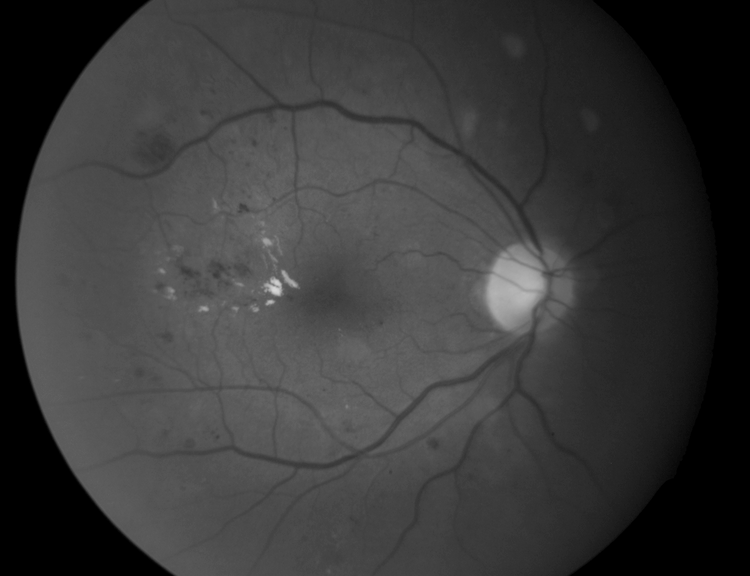
\includegraphics[width=\linewidth]{chap05_disease_green}
    \caption{Extrahovaný zelený kanál.}
    \label{pic:chap05_disease_green}
  \end{minipage}
\end{figure}

\begin{figure}[h]
  \begin{minipage}[c]{0.47\textwidth}
    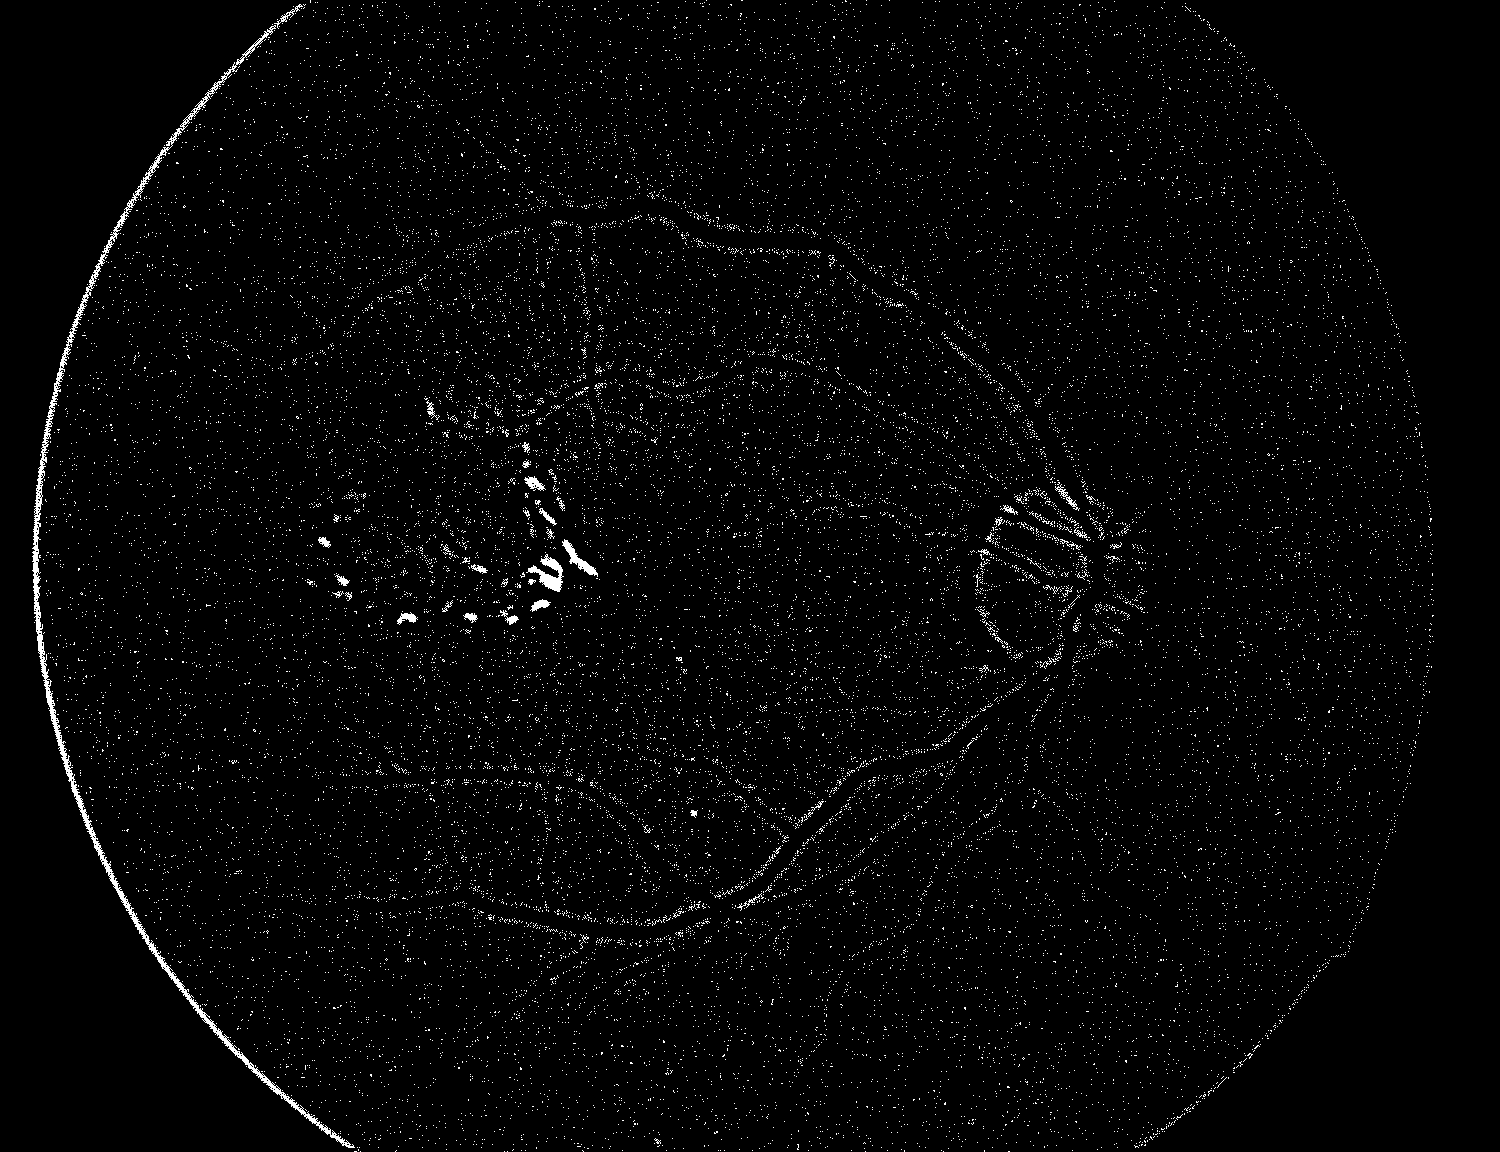
\includegraphics[width=\linewidth]{chap05_disease_threshold}
    \caption{Výsledek prahování.}
    \label{pic:chap05_disease_threshold}
  \end{minipage}
  \hfill
  \begin{minipage}[c]{0.47\textwidth}
    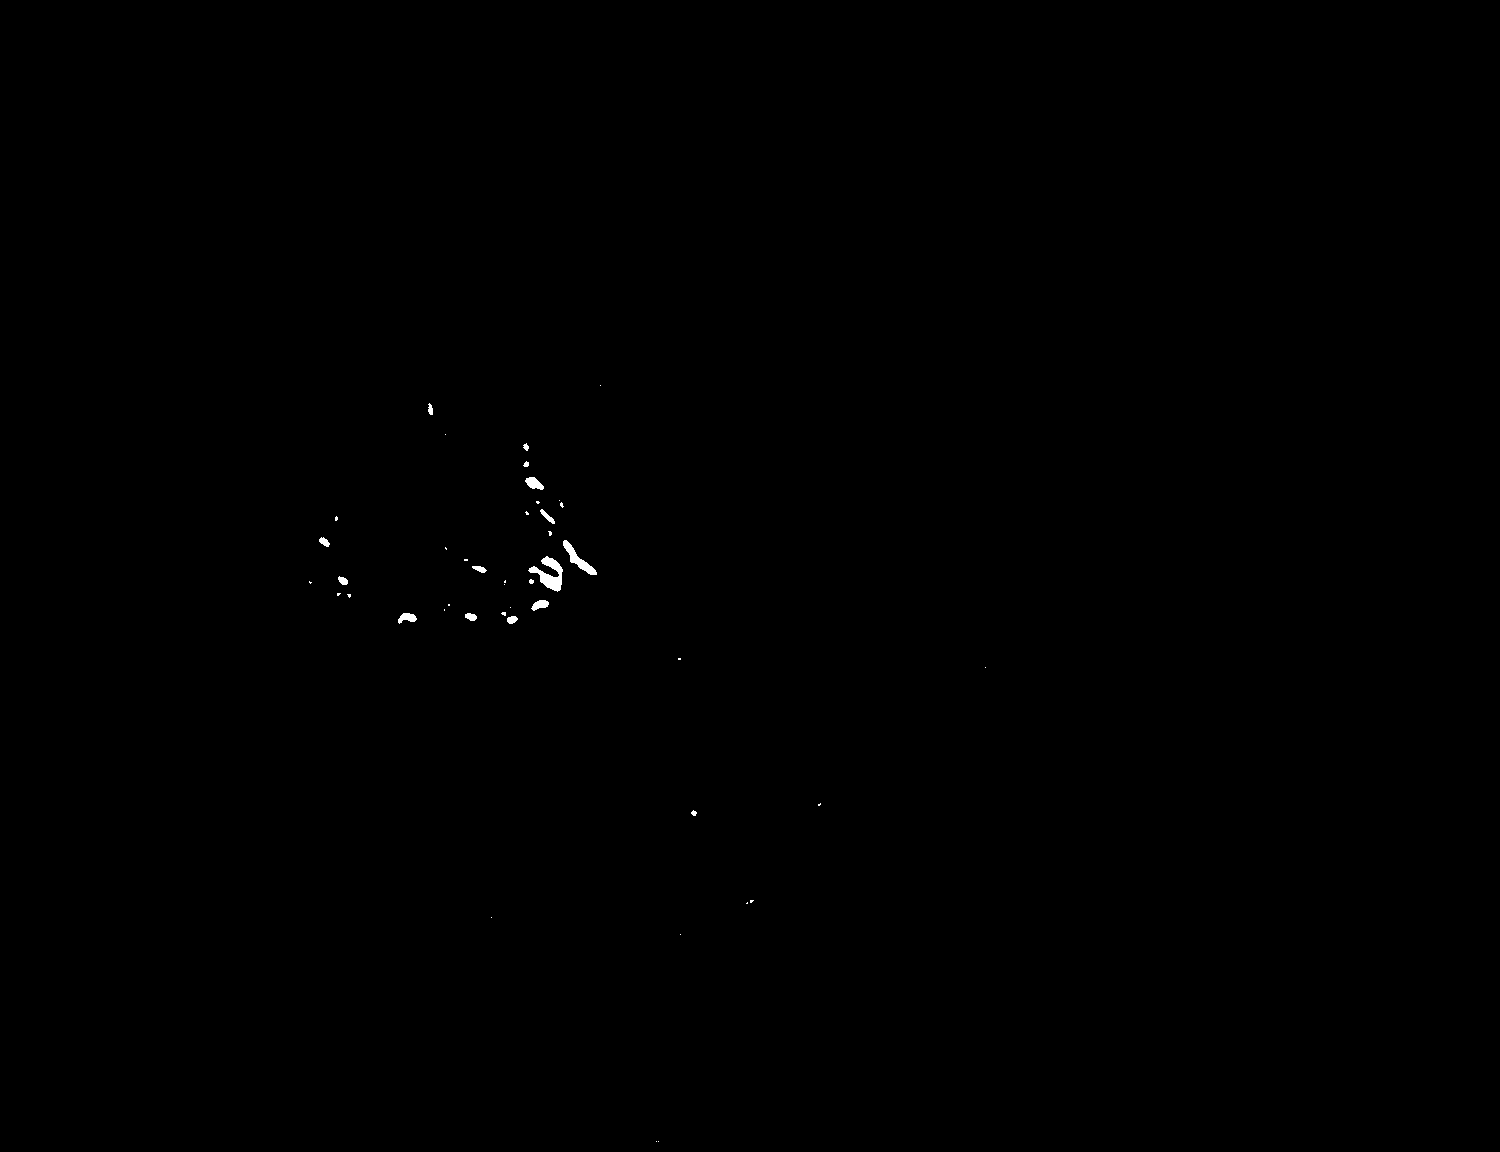
\includegraphics[width=\linewidth]{chap05_disease_suspect}
    \caption{Získané podezřelé oblasti.}
    \label{pic:chap05_disease_suspect}
  \end{minipage}
\end{figure}


\subsection*{Úprava masky krevního řečiště}
Snímky sítnic, jejichž krevní řečiště velmi dobře kontrastuje s~pozadím sítnice, způsobí, že obrysy těchto cév se zahrnou do podezřelých oblastí. Aby se tomu zabránilo, je potřeba provést úpravu masky krevního řečiště ještě před jejím použitím. Úprava představuje dilataci této masky, aby došlo k~rozšíření daných cév. Rozdíl mezi původní a dilatovanou maskou je zobrazen na obrázcích \ref{pic:chap05_disease_vessel_mask} a \ref{pic:chap05_disease_vessel_mask_dilated}. Jakmile se tato maska aplikuje, vyloučí se ze zpracovávaného snímku nežádoucí obrysy. Porovnání mezi podezřelými oblastmi, na nichž se použila neupravená a upravená maska, lze vidět na obrázcích \ref{pic:chap05_disease_suspect_unchanged} a \ref{pic:chap05_disease_suspect_changed}.

\begin{figure}[h]
  \begin{minipage}[c]{0.47\textwidth}
    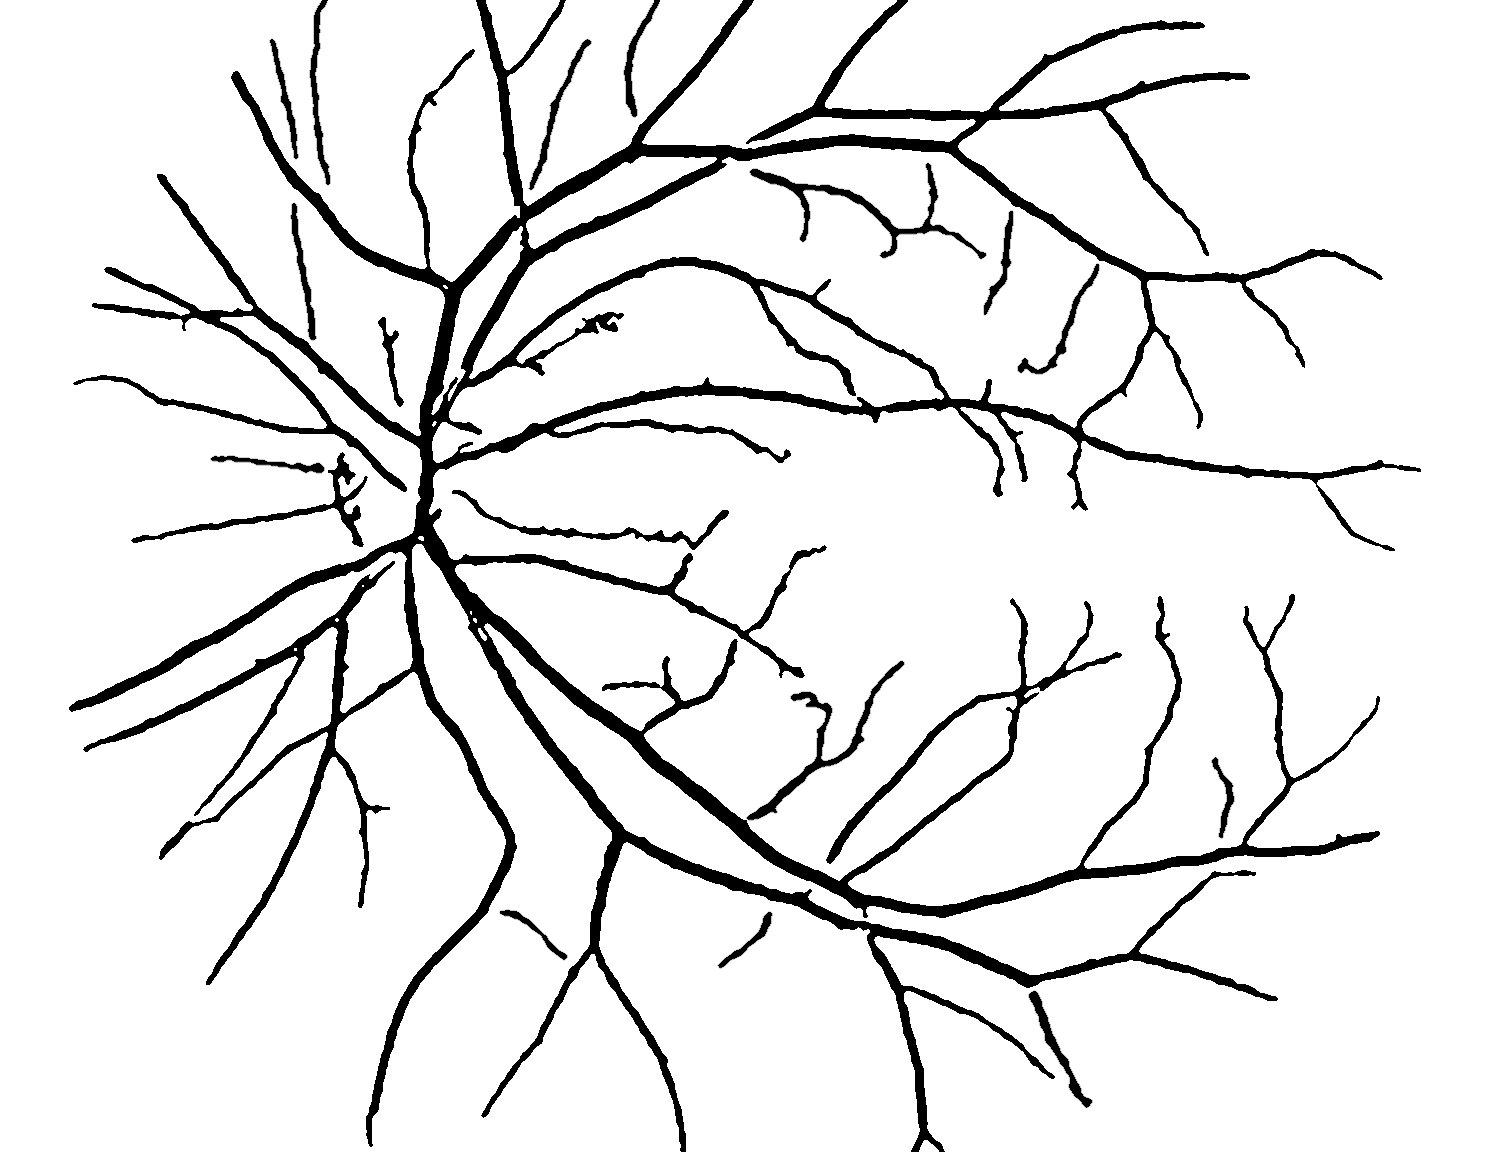
\includegraphics[width=\linewidth]{chap05_disease_vessel_mask}
    \caption{Původní maska.}
    \label{pic:chap05_disease_vessel_mask}
  \end{minipage}
  \hfill
  \begin{minipage}[c]{0.47\textwidth}
    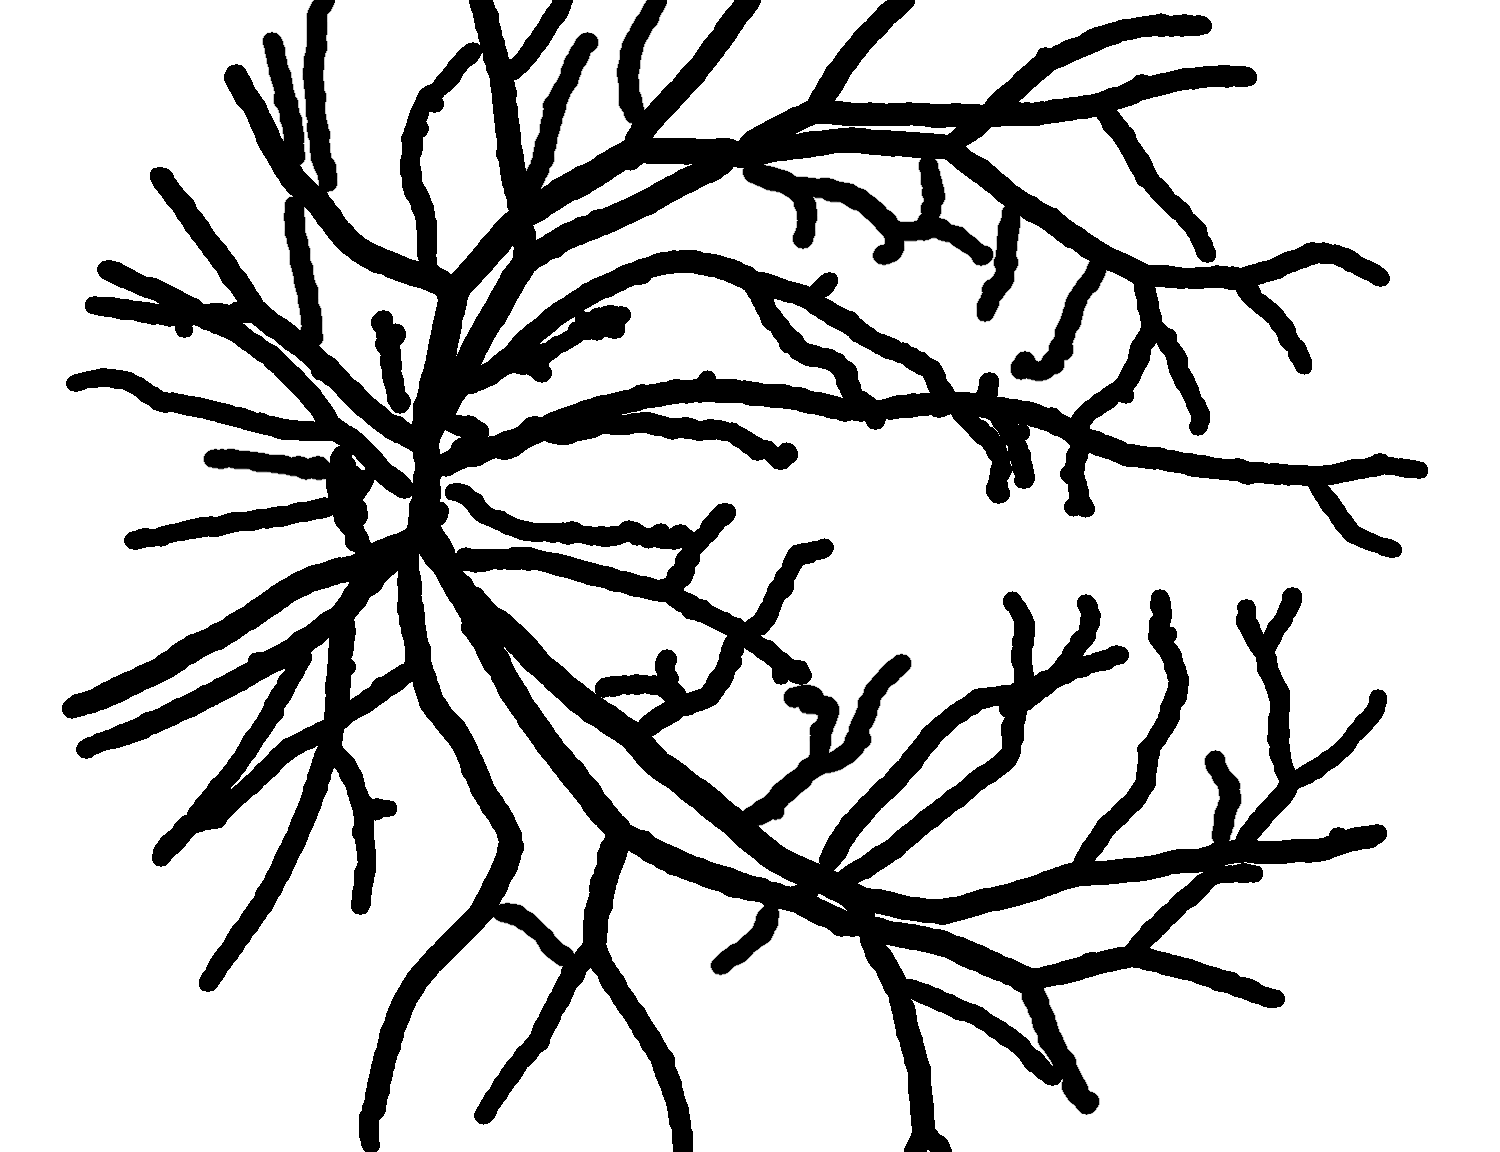
\includegraphics[width=\linewidth]{chap05_disease_vessel_mask_dilated}
    \caption{Maska po dilataci.}
    \label{pic:chap05_disease_vessel_mask_dilated}
  \end{minipage}
\end{figure}

\begin{figure}[h]
  \begin{minipage}[c]{0.47\textwidth}
    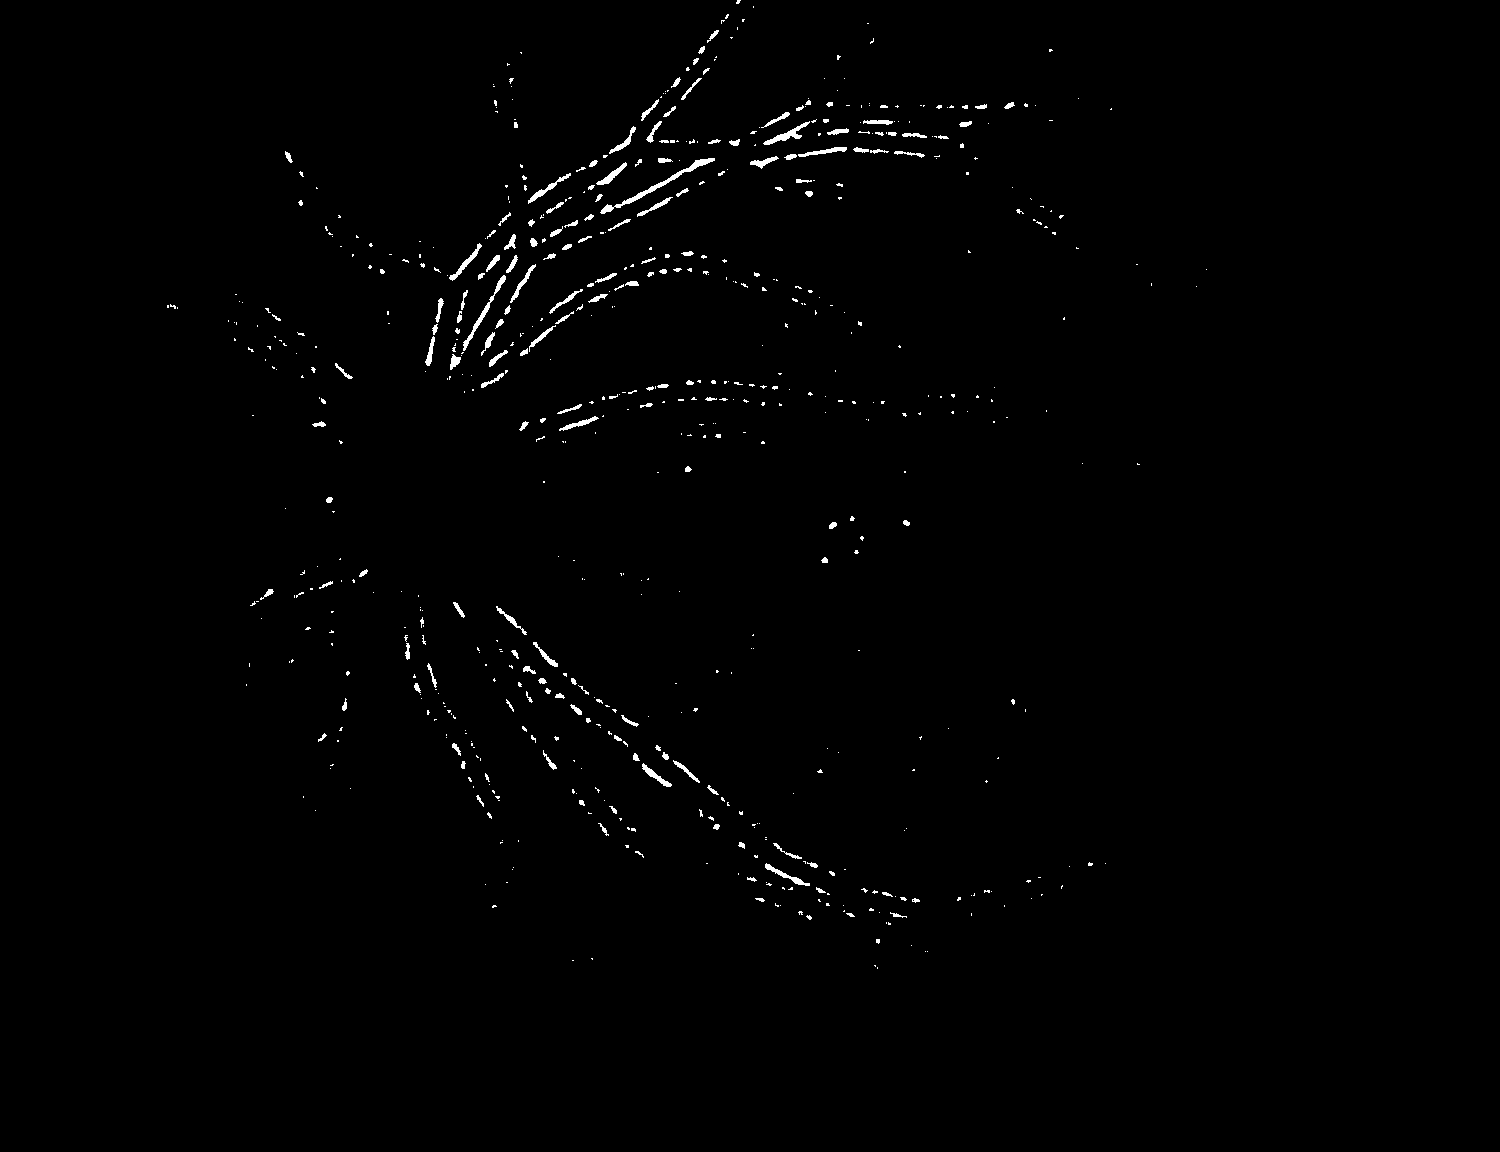
\includegraphics[width=\linewidth]{chap05_disease_suspect_unchanged}
    \caption{Podezřelé oblasti s~neupravenou maskou.}
    \label{pic:chap05_disease_suspect_unchanged}
  \end{minipage}
  \hfill
  \begin{minipage}[c]{0.47\textwidth}
    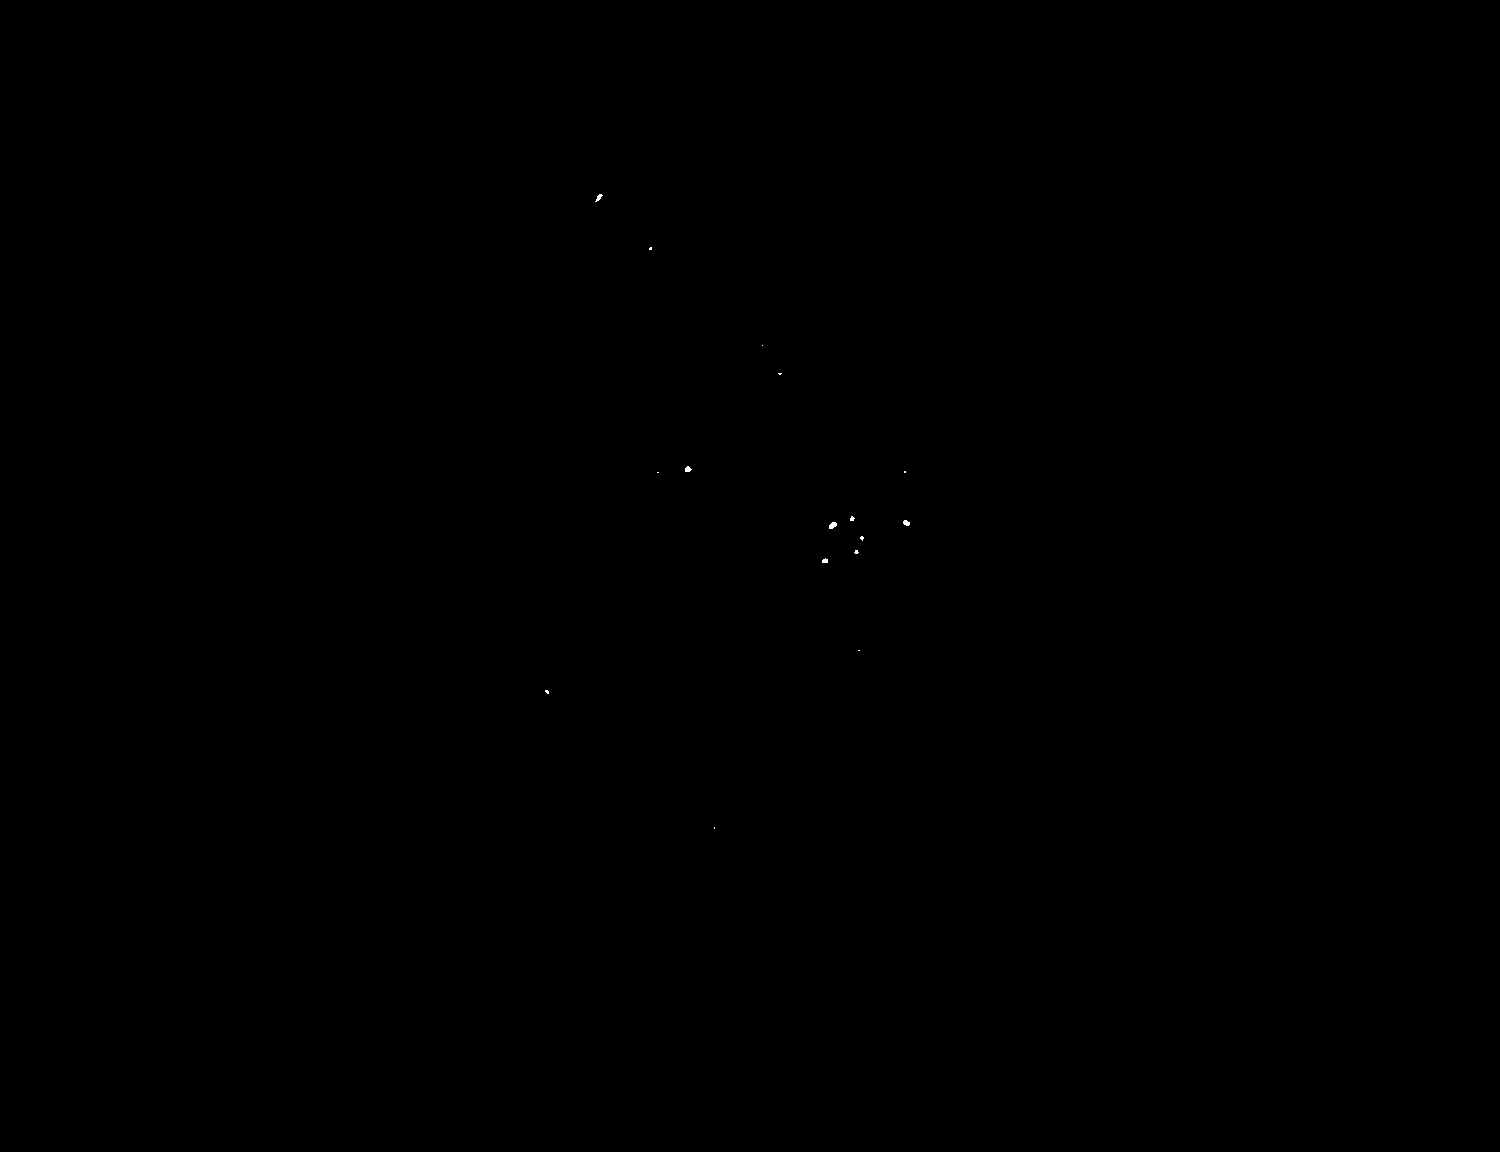
\includegraphics[width=\linewidth]{chap05_disease_suspect_changed}
    \caption{Podezřelé oblasti s~upravenou maskou.}
    \label{pic:chap05_disease_suspect_changed}
  \end{minipage}
\end{figure}


\subsection*{Klasifikace podezřelých oblastí}
Posledním krokem je určit, které z~vymezených podezřelých oblastí představují drúzy či exudáty a které naopak ne. K~tomuto účelu se využívá HSV barevného modelu, do kterého je vstupní snímek převeden. HSV barevný model se skládá ze tří složek, kterými jsou: barevný tón (hue), sytost barvy (saturation) a hodnota jasu (value) neboli množství bílého světla v~obraze.

Nejprve se naleznou obrysy podezřelých oblastí, na jejichž základě se vypočítají jejich obsahy. Pokud je obsah dané plochy větší než 3~pixely, lokalizuje se odpovídající plocha v~HSV obrázku. Z~toho lze následně vypočítat průměrnou hodnotu barevného tónu, sytost a jas této oblasti. Experimentováním nad různými obrázky byly vytyčeny meze, které jsou uvedeny v~tabulce \ref{tab:hsv_color_limits}. Pokud některá z~oblastí spadá do jedné z~těchto mezí, jedná se o~drúzu nebo exudát.

\begin{table}[ht]
  \begin{center}	
    \begin{tabular}{|c|c|c|c|}
      \hline
      Hodnota & Mez 1 & Mez 2   & Mez 3 \\
      \hline
      H & 30--12   &  30--15 &  30--19 \\
      \hline
      S~& 255--170 & 255--120 & 255--187 \\
      \hline
      V~& 255--120 & 255--84 & 255--75 \\
      \hline
    \end{tabular}
  \caption{Přehled HSV mezí pro klasifikaci podezřelých oblastí.}
  \label{tab:hsv_color_limits}
  \end{center}
\end{table}

Jakmile byla oblast klasifikována jako nález, vypočítá se pomocí matematických momentů její těžiště, které představuje střed, ze kterého se vytvoří kružnice pro označení nálezu. Značení se nejprve provádí do prázdného snímku, ze kterého jsou po zkontrolování všech oblastí vybrány externí obrysy. Ty jsou zakresleny do výsledného obrázku, aby jednotlivé kružnice nepřekrývaly detekované nálezy. Výsledek detekce lze vidět na obrázku \ref{pic:chap05_disease_result}.

\begin{figure}[h]
  \begin{center}
    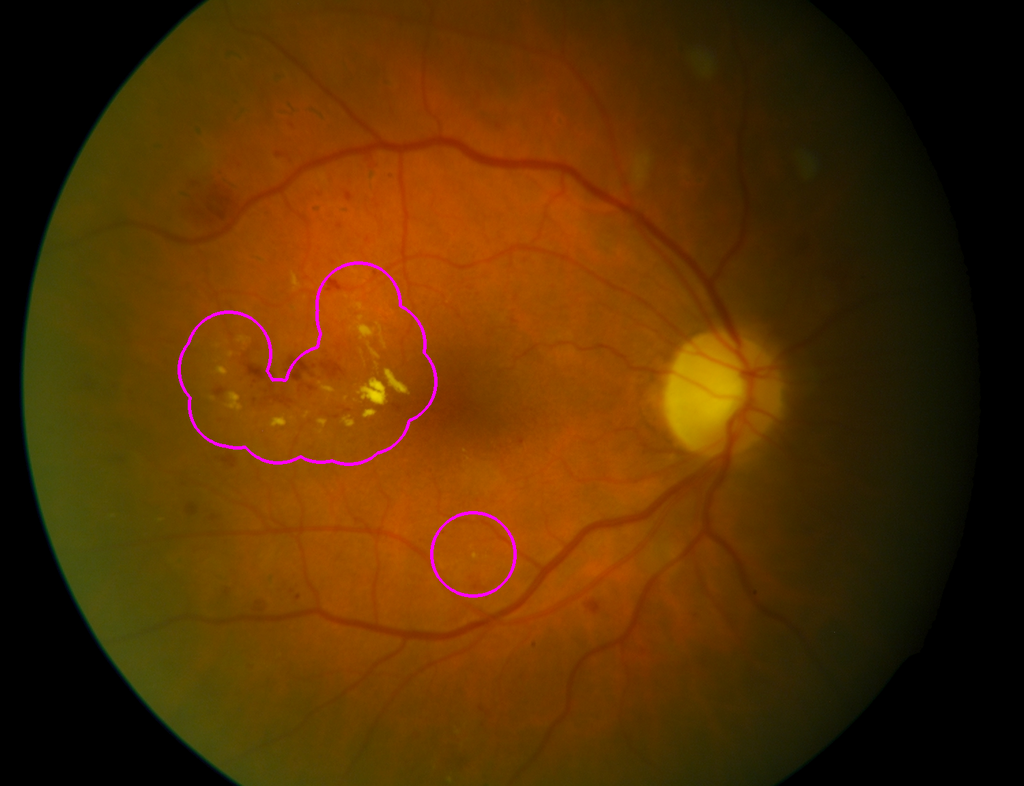
\includegraphics[width=.75\linewidth]{chap05_disease_result}
    \caption{Výsledek detekce.}
    \label{pic:chap05_disease_result}
  \end{center}
\end{figure}


\section{Výsledná struktura programu}
Navržený program pro automatickou detekci příznaků VPMD je implementován v~programovacím jazyce C++ s~využitím knihovny OpenCV. Mezi hlavní výhody této knihovny patří velké množství funkcí pro zpracování obrazu, které v~sobě zahrnuje, přenositelnost mezi různými operačními systémy a její volnou dostupnost pro akademické i komerční účely.

Výsledný program je rozdělen do několika souborů. Soubory \emph{detection.h} a \emph{detection.cpp} obsahují funkce implementující algoritmy, které byly navrženy výše. V~souborech \emph{tester.h} a \emph{tester.cpp} je implementována třída \emph{Tester} pro účely testování. Následující kapitola \ref{ch:testovani} obsahuje podrobnější popis funkce této třídy. Poslední hlavní soubor \emph{main.cpp} představuje vstupní bod programu, kde se zpracovávají vstupní argumenty, na jejichž základě se odvíjí další provádění programu.\par 

\bigskip\bigskip
\noindent\textbf{Přehled vstupních argumentů}\par\bigskip

\begin{tabularx}{\textwidth}{p{4cm}X}
  \textbf{-h, {-}{-}help}               & zobrazí nápovědu \\[5mm]
  \textbf{-i, {-}{-}image} \emph{path}   & vstupní snímek pro zpracování umístěný v~\emph{path} \\[5mm]
  \textbf{-d, {-}{-}detect}             & detekuje drúzy a exudáty \\[5mm]
  \textbf{{-}{-}mark}                   & vyznačí oblast optického disku a fovey \\[5mm]
  \textbf{{-}{-}mask}                   & zobrazí masku pozadí, optického disku a cév v~jediném snímku \\[5mm]
  \textbf{{-}{-}collect} \emph{database} & manuální lokalizace optického disku a fovey ve snímcích databáze \emph{database} pro vytvoření souboru \emph{groundtruth}\\[5mm]
  \textbf{{-}{-}test} \emph{groundtruth} & spuštění automatického testování detekce optického disku a fovey nad souborem \emph{groundtruth} \\[5mm]
  \textbf{{-}{-}compare} \emph{database} & postupné zobrazení všech snímků v~databázi \emph{database} a k~nim odpovídajících snímků s~detekovanými nálezy pro porovnání \\[5mm]
\end{tabularx}

\bigskip\bigskip
\noindent\textbf{Příklady spuštění}\par\bigskip

\begingroup
\setlength{\tabcolsep}{0pt}
\noindent\begin{tabularx}{\textwidth}{p{8.5cm}X}
  \emph{.{/}detector -i image001.png {-}{-}mask}               & zobrazí vstupní snímek spolu s~vytvořenou masku\\[5mm]
  \emph{.{/}detector -i image002.png {-}{-}mark {-}{-}detect}  & zobrazí vstupní snímek spolu se snímkem, na kterém je zaznačen optický disk, fovea a detekované nálezy\\[5mm]
  \emph{.{/}detector {-}{-}collect database{/}FIRE}            & vytvoří soubor \emph{groundtruth} v~adresáři databáze po manuální lokalizaci optického disku a fovey uživatelem\\[5mm]
  \emph{.{/}detector {-}{-}test database{/}FIRE{/}groundtruth} & spustí automatické testování ze souboru \emph{groundtruth} a do stejného adresáře vytvoří soubor \emph{test\_results} obsahující výsledky testování\\[5mm]
\end{tabularx}
\endgroup